%%%%%%%%%%%%%%%%%%%%%%%%%%%%%%%%%%%%%%%%%
% The Legrand Orange Book
% LaTeX Template
% Version 2.0 (9/2/15)
%
% This template has been downloaded from:
% http://www.LaTeXTemplates.com
%
% Mathias Legrand (legrand.mathias@gmail.com) with modifications by:
% Vel (vel@latextemplates.com)
%
% License:
% CC BY-NC-SA 3.0 (http://creativecommons.org/licenses/by-nc-sa/3.0/)
%
% Compiling this template:
% This template uses biber for its bibliography and makeindex for its index.
% When you first open the template, compile it from the command line with the 
% commands below to make sure your LaTeX distribution is configured correctly:
%
% 1) pdflatex main
% 2) makeindex main.idx -s StyleInd.ist
% 3) biber main
% 4) pdflatex main x 2
%
% After this, when you wish to update the bibliography/index use the appropriate
% command above and make sure to compile with pdflatex several times 
% afterwards to propagate your changes to the document.
%
% This template also uses a number of packages which may need to be
% updated to the newest versions for the template to compile. It is strongly
% recommended you update your LaTeX distribution if you have any
% compilation errors.
%
% Important note:
% Chapter heading images should have a 2:1 width:height ratio,
% e.g. 920px width and 460px height.
%
%%%%%%%%%%%%%%%%%%%%%%%%%%%%%%%%%%%%%%%%%

%----------------------------------------------------------------------------------------
%	PACKAGES AND OTHER DOCUMENT CONFIGURATIONS
%----------------------------------------------------------------------------------------

\documentclass[12pt,fleqn]{book} % Default font size and left-justified equations
%\setlength{\parskip}{0.15cm}
%\setlength{\parindent}{0pt}

%----------------------------------------------------------------------------------------

%%%%%%%%%%%%%%%%%%%%%%%%%%%%%%%%%%%%%%%%%
% The Legrand Orange Book
% Structural Definitions File
% Version 2.0 (9/2/15)
%
% Original author:
% Mathias Legrand (legrand.mathias@gmail.com) with modifications by:
% Vel (vel@latextemplates.com)
% 
% This file has been downloaded from:
% http://www.LaTeXTemplates.com
%
% License:
% CC BY-NC-SA 3.0 (http://creativecommons.org/licenses/by-nc-sa/3.0/)
%
%%%%%%%%%%%%%%%%%%%%%%%%%%%%%%%%%%%%%%%%%

%----------------------------------------------------------------------------------------
%	VARIOUS REQUIRED PACKAGES AND CONFIGURATIONS
%----------------------------------------------------------------------------------------

\usepackage[top=3cm,bottom=3cm,left=3cm,right=3cm,headsep=10pt,a4paper,marginparwidth=2cm]{geometry} % Page margins

\usepackage{graphicx,import} % Required for including pictures
\graphicspath{{Pictures/}} % Specifies the directory where pictures are stored

\usepackage{lipsum} % Inserts dummy text

\usepackage{tikz} % Required for drawing custom shapes

\usepackage[english]{babel} % English language/hyphenation

\usepackage{enumitem} % Customize lists
\setlist{nolistsep} % Reduce spacing between bullet points and numbered lists

\usepackage{booktabs} % Required for nicer horizontal rules in tables

\usepackage{xcolor} % Required for specifying colors by name
\definecolor{ocre}{RGB}{243,102,25} % Define the orange color used for highlighting throughout the book

% added by Frank
\usepackage{float}
\usepackage{units}
\usepackage[]{algorithm2e}
\usepackage{marginnote}
\usepackage{stmaryrd}
\usepackage{wrapfig}
\usepackage{soul}
\usepackage{cancel}

%----------------------------------------------------------------------------------------
%	FONTS
%----------------------------------------------------------------------------------------

\usepackage{avant} % Use the Avantgarde font for headings
%\usepackage{times} % Use the Times font for headings
\usepackage{mathptmx} % Use the Adobe Times Roman as the default text font together with math symbols from the Sym­bol, Chancery and Com­puter Modern fonts

\usepackage{microtype} % Slightly tweak font spacing for aesthetics
\usepackage[utf8]{inputenc} % Required for including letters with accents
\usepackage[T1]{fontenc} % Use 8-bit encoding that has 256 glyphs

%----------------------------------------------------------------------------------------
%	BIBLIOGRAPHY AND INDEX
%----------------------------------------------------------------------------------------

\usepackage[style=alphabetic,citestyle=numeric,sorting=nyt,sortcites=true,autopunct=true,babel=hyphen,hyperref=true,abbreviate=false,backref=true,backend=biber]{biblatex}
\addbibresource{bibliography.bib} % BibTeX bibliography file
\defbibheading{bibempty}{}

\usepackage{calc} % For simpler calculation - used for spacing the index letter headings correctly
\usepackage{makeidx} % Required to make an index
\makeindex % Tells LaTeX to create the files required for indexing

%----------------------------------------------------------------------------------------
%	MAIN TABLE OF CONTENTS
%----------------------------------------------------------------------------------------

\usepackage{titletoc} % Required for manipulating the table of contents

\contentsmargin{0cm} % Removes the default margin

% Part text styling
\titlecontents{part}[0cm]
{\addvspace{20pt}\centering\large\bfseries}
{}
{}
{}

% Chapter text styling
\titlecontents{chapter}[1.25cm] % Indentation
{\addvspace{12pt}\large\sffamily\bfseries} % Spacing and font options for chapters
{\color{ocre!60}\contentslabel[\Large\thecontentslabel]{1.25cm}\color{ocre}} % Chapter number
{\color{ocre}}  
{\color{ocre!60}\normalsize\;\titlerule*[.5pc]{.}\;\thecontentspage} % Page number

% Section text styling
\titlecontents{section}[1.25cm] % Indentation
{\addvspace{3pt}\sffamily\bfseries} % Spacing and font options for sections
{\contentslabel[\thecontentslabel]{1.25cm}} % Section number
{}
{\hfill\color{black}\thecontentspage} % Page number
[]

% Subsection text styling
\titlecontents{subsection}[1.25cm] % Indentation
{\addvspace{1pt}\sffamily\small} % Spacing and font options for subsections
{\contentslabel[\thecontentslabel]{1.25cm}} % Subsection number
{}
{\ \titlerule*[.5pc]{.}\;\thecontentspage} % Page number
[]

% List of figures
\titlecontents{figure}[0em]
{\addvspace{-5pt}\sffamily}
{\thecontentslabel\hspace*{1em}}
{}
{\ \titlerule*[.5pc]{.}\;\thecontentspage}
[]

% List of tables
\titlecontents{table}[0em]
{\addvspace{-5pt}\sffamily}
{\thecontentslabel\hspace*{1em}}
{}
{\ \titlerule*[.5pc]{.}\;\thecontentspage}
[]

%----------------------------------------------------------------------------------------
%	MINI TABLE OF CONTENTS IN PART HEADS
%----------------------------------------------------------------------------------------

% Chapter text styling
\titlecontents{lchapter}[0em] % Indenting
{\addvspace{15pt}\large\sffamily\bfseries} % Spacing and font options for chapters
{\color{ocre}\contentslabel[\Large\thecontentslabel]{1.25cm}\color{ocre}} % Chapter number
{}  
{\color{ocre}\normalsize\sffamily\bfseries\;\titlerule*[.5pc]{.}\;\thecontentspage} % Page number

% Section text styling
\titlecontents{lsection}[0em] % Indenting
{\sffamily\small} % Spacing and font options for sections
{\contentslabel[\thecontentslabel]{1.25cm}} % Section number
{}
{}

% Subsection text styling
\titlecontents{lsubsection}[.5em] % Indentation
{\normalfont\footnotesize\sffamily} % Font settings
{}
{}
{}

%----------------------------------------------------------------------------------------
%	PAGE HEADERS
%----------------------------------------------------------------------------------------

\usepackage{fancyhdr} % Required for header and footer configuration

\pagestyle{fancy}
\renewcommand{\chaptermark}[1]{\markboth{\sffamily\normalsize\bfseries\chaptername\ \thechapter.\ #1}{}} % Chapter text font settings
\renewcommand{\sectionmark}[1]{\markright{\sffamily\normalsize\thesection\hspace{5pt}#1}{}} % Section text font settings
\fancyhf{} \fancyhead[LE,RO]{\sffamily\normalsize\thepage} % Font setting for the page number in the header
\fancyhead[LO]{\rightmark} % Print the nearest section name on the left side of odd pages
\fancyhead[RE]{\leftmark} % Print the current chapter name on the right side of even pages
\renewcommand{\headrulewidth}{0.5pt} % Width of the rule under the header
\addtolength{\headheight}{2.5pt} % Increase the spacing around the header slightly
\renewcommand{\footrulewidth}{0pt} % Removes the rule in the footer
\fancypagestyle{plain}{\fancyhead{}\renewcommand{\headrulewidth}{0pt}} % Style for when a plain pagestyle is specified

% Removes the header from odd empty pages at the end of chapters
\makeatletter
\renewcommand{\cleardoublepage}{
\clearpage\ifodd\c@page\else
\hbox{}
\vspace*{\fill}
\thispagestyle{empty}
\newpage
\fi}

%----------------------------------------------------------------------------------------
%	THEOREM STYLES
%----------------------------------------------------------------------------------------

\usepackage{amsmath,amsfonts,amssymb,amsthm} % For math equations, theorems, symbols, etc

\newcommand{\intoo}[2]{\mathopen{]}#1\,;#2\mathclose{[}}
\newcommand{\ud}{\mathop{\mathrm{{}d}}\mathopen{}}
\newcommand{\intff}[2]{\mathopen{[}#1\,;#2\mathclose{]}}

% Boxed/framed environments
\newtheoremstyle{ocrenumbox}% % Theorem style name
{0pt}% Space above
{0pt}% Space below
{\normalfont}% % Body font
{}% Indent amount
{\small\bf\sffamily\color{ocre}}% % Theorem head font
{\;}% Punctuation after theorem head
{0.25em}% Space after theorem head
{\small\sffamily\color{ocre}\thmname{#1}\nobreakspace\thmnumber{\@ifnotempty{#1}{}\@upn{#2}}% Theorem text (e.g. Theorem 2.1)
\thmnote{\nobreakspace\the\thm@notefont\sffamily\bfseries\color{black}---\nobreakspace#3.}} % Optional theorem note
\renewcommand{\qedsymbol}{$\blacksquare$}% Optional qed square

\newtheoremstyle{blacknumex}% Theorem style name
{5pt}% Space above
{5pt}% Space below
{\normalfont}% Body font
{} % Indent amount
{\small\bf\sffamily}% Theorem head font
{\;}% Punctuation after theorem head
{0.25em}% Space after theorem head
{\small\sffamily{\tiny\ensuremath{\blacksquare}}\nobreakspace\thmname{#1}\nobreakspace\thmnumber{\@ifnotempty{#1}{}\@upn{#2}}% Theorem text (e.g. Theorem 2.1)
\thmnote{\nobreakspace\the\thm@notefont\sffamily\bfseries---\nobreakspace#3.}}% Optional theorem note

\newtheoremstyle{blacknumbox} % Theorem style name
{0pt}% Space above
{0pt}% Space below
{\normalfont}% Body font
{}% Indent amount
{\small\bf\sffamily}% Theorem head font
{\;}% Punctuation after theorem head
{0.25em}% Space after theorem head
{\small\sffamily\thmname{#1}\nobreakspace\thmnumber{\@ifnotempty{#1}{}\@upn{#2}}% Theorem text (e.g. Theorem 2.1)
\thmnote{\nobreakspace\the\thm@notefont\sffamily\bfseries---\nobreakspace#3.}}% Optional theorem note

% Non-boxed/non-framed environments
\newtheoremstyle{ocrenum}% % Theorem style name
{5pt}% Space above
{5pt}% Space below
{\normalfont}% % Body font
{}% Indent amount
{\small\bf\sffamily\color{ocre}}% % Theorem head font
{\;}% Punctuation after theorem head
{0.25em}% Space after theorem head
{\small\sffamily\color{ocre}\thmname{#1}\nobreakspace\thmnumber{\@ifnotempty{#1}{}\@upn{#2}}% Theorem text (e.g. Theorem 2.1)
\thmnote{\nobreakspace\the\thm@notefont\sffamily\bfseries\color{black}---\nobreakspace#3.}} % Optional theorem note
\renewcommand{\qedsymbol}{$\blacksquare$}% Optional qed square
\makeatother

% Defines the theorem text style for each type of theorem to one of the three styles above
\newcounter{dummy} 
\newtheorem{notation}[dummy]{Notation}
\numberwithin{dummy}{chapter}
\theoremstyle{ocrenumbox}
\newtheorem{theoremeT}[dummy]{Theorem}
\newtheorem{problem}[dummy]{Problem}
\newtheorem{exerciseT}[dummy]{Exercise}
\theoremstyle{blacknumex}
\newtheorem{exampleT}[dummy]{Example}
\theoremstyle{blacknumbox}
\newtheorem{vocabulary}[dummy]{Vocabulary}
\newtheorem{definitionT}[dummy]{Definition}
\newtheorem{lemmaT}[dummy]{Lemma}
\theoremstyle{ocrenum}
\newtheorem{proposition}[dummy]{Proposition}


%----------------------------------------------------------------------------------------
%	DEFINITION OF COLORED BOXES
%----------------------------------------------------------------------------------------

\RequirePackage[framemethod=default]{mdframed} % Required for creating the theorem, definition, exercise and lemma boxes

% Theorem box
\newmdenv[skipabove=7pt,
skipbelow=7pt,
backgroundcolor=black!5,
linecolor=ocre,
innerleftmargin=5pt,
innerrightmargin=5pt,
innertopmargin=5pt,
leftmargin=0cm,
rightmargin=0cm,
innerbottommargin=5pt]{tBox}

% Exercise box	  
\newmdenv[skipabove=7pt,
skipbelow=7pt,
rightline=false,
leftline=true,
topline=false,
bottomline=false,
backgroundcolor=ocre!10,
linecolor=ocre,
innerleftmargin=5pt,
innerrightmargin=5pt,
innertopmargin=5pt,
innerbottommargin=5pt,
leftmargin=0cm,
rightmargin=0cm,
linewidth=4pt]{eBox}	

% Definition box
\newmdenv[skipabove=7pt,
skipbelow=7pt,
rightline=false,
leftline=true,
topline=false,
bottomline=false,
linecolor=ocre,
innerleftmargin=5pt,
innerrightmargin=5pt,
innertopmargin=0pt,
leftmargin=0cm,
rightmargin=0cm,
linewidth=4pt,
innerbottommargin=0pt]{dBox}	

% Lemma box
\newmdenv[skipabove=7pt,
skipbelow=7pt,
rightline=false,
leftline=true,
topline=false,
bottomline=false,
linecolor=gray,
backgroundcolor=black!5,
innerleftmargin=5pt,
innerrightmargin=5pt,
innertopmargin=5pt,
leftmargin=0cm,
rightmargin=0cm,
linewidth=4pt,
innerbottommargin=5pt]{cBox}

% Creates an environment for each type of theorem and assigns it a theorem text style from the "Theorem Styles" section above and a colored box from above
\newenvironment{theorem}{\begin{tBox}\begin{theoremeT}}{\end{theoremeT}\end{tBox}}
\newenvironment{exercise}{\begin{eBox}\begin{exerciseT}}{\hfill{\color{ocre}\tiny\ensuremath{\blacksquare}}\end{exerciseT}\end{eBox}}				  
\newenvironment{definition}{\begin{dBox}\begin{definitionT}}{\end{definitionT}\end{dBox}}	
\newenvironment{example}{\begin{exampleT}}{\hfill{\tiny\ensuremath{\blacksquare}}\end{exampleT}}		
\newenvironment{lemma}{\begin{cBox}\begin{lemmaT}}{\end{lemmaT}\end{cBox}}	

%----------------------------------------------------------------------------------------
%	REMARK ENVIRONMENT
%----------------------------------------------------------------------------------------

\newenvironment{remark}{\par\vspace{10pt}\small % Vertical white space above the remark and smaller font size
\begin{list}{}{
\leftmargin=35pt % Indentation on the left
\rightmargin=25pt}\item\ignorespaces % Indentation on the right
\makebox[-2.5pt]{
\begin{tikzpicture}[overlay]
\node[draw=ocre!60,line width=1pt,circle,fill=ocre!25,font=\sffamily\bfseries,inner sep=2pt,outer sep=0pt] at (-15pt,0pt){\textcolor{ocre}{R}};\end{tikzpicture}} % Orange R in a circle
\advance\baselineskip -1pt}{\end{list}\vskip5pt} % Tighter line spacing and white space after remark

%----------------------------------------------------------------------------------------
%	SECTION NUMBERING IN THE MARGIN
%----------------------------------------------------------------------------------------

\makeatletter
\renewcommand{\@seccntformat}[1]{\llap{\textcolor{ocre}{\csname the#1\endcsname}\hspace{1em}}}                    
\renewcommand{\section}{\@startsection{section}{1}{\z@}
{-4ex \@plus -1ex \@minus -.4ex}
{1ex \@plus.2ex }
{\normalfont\large\sffamily\bfseries}}
\renewcommand{\subsection}{\@startsection {subsection}{2}{\z@}
{-3ex \@plus -0.1ex \@minus -.4ex}
{0.5ex \@plus.2ex }
{\normalfont\sffamily\bfseries}}
\renewcommand{\subsubsection}{\@startsection {subsubsection}{3}{\z@}
{-2ex \@plus -0.1ex \@minus -.2ex}
{.2ex \@plus.2ex }
{\normalfont\small\sffamily\bfseries}}                        
\renewcommand\paragraph{\@startsection{paragraph}{4}{\z@}
{-2ex \@plus-.2ex \@minus .2ex}
{.1ex}
{\normalfont\small\sffamily\bfseries}}

%----------------------------------------------------------------------------------------
%	PART HEADINGS
%----------------------------------------------------------------------------------------

% numbered part in the table of contents
\newcommand{\@mypartnumtocformat}[2]{%
\setlength\fboxsep{0pt}%
\noindent\colorbox{ocre!20}{\strut\parbox[c][.7cm]{\ecart}{\color{ocre!70}\Large\sffamily\bfseries\centering#1}}\hskip\esp\colorbox{ocre!40}{\strut\parbox[c][.7cm]{\linewidth-\ecart-\esp}{\Large\sffamily\centering#2}}}%
%%%%%%%%%%%%%%%%%%%%%%%%%%%%%%%%%%
% unnumbered part in the table of contents
\newcommand{\@myparttocformat}[1]{%
\setlength\fboxsep{0pt}%
\noindent\colorbox{ocre!40}{\strut\parbox[c][.7cm]{\linewidth}{\Large\sffamily\centering#1}}}%
%%%%%%%%%%%%%%%%%%%%%%%%%%%%%%%%%%
\newlength\esp
\setlength\esp{4pt}
\newlength\ecart
\setlength\ecart{1.2cm-\esp}
\newcommand{\thepartimage}{}%
\newcommand{\partimage}[1]{\renewcommand{\thepartimage}{#1}}%
\def\@part[#1]#2{%
\ifnum \c@secnumdepth >-2\relax%
\refstepcounter{part}%
\addcontentsline{toc}{part}{\texorpdfstring{\protect\@mypartnumtocformat{\thepart}{#1}}{\partname~\thepart\ ---\ #1}}
\else%
\addcontentsline{toc}{part}{\texorpdfstring{\protect\@myparttocformat{#1}}{#1}}%
\fi%
\startcontents%
\markboth{}{}%
{\thispagestyle{empty}%
\begin{tikzpicture}[remember picture,overlay]%
\node at (current page.north west){\begin{tikzpicture}[remember picture,overlay]%	
\fill[ocre!20](0cm,0cm) rectangle (\paperwidth,-\paperheight);
\node[anchor=north] at (4cm,-3.25cm){\color{ocre!40}\fontsize{220}{100}\sffamily\bfseries\@Roman\c@part}; 
\node[anchor=south east] at (\paperwidth-1cm,-\paperheight+1cm){\parbox[t][][t]{8.5cm}{
\printcontents{l}{0}{\setcounter{tocdepth}{1}}%
}};
\node[anchor=north east] at (\paperwidth-1.5cm,-3.25cm){\parbox[t][][t]{15cm}{\strut\raggedleft\color{white}\fontsize{30}{30}\sffamily\bfseries#2}};
\end{tikzpicture}};
\end{tikzpicture}}%
\@endpart}
\def\@spart#1{%
\startcontents%
\phantomsection
{\thispagestyle{empty}%
\begin{tikzpicture}[remember picture,overlay]%
\node at (current page.north west){\begin{tikzpicture}[remember picture,overlay]%	
\fill[ocre!20](0cm,0cm) rectangle (\paperwidth,-\paperheight);
\node[anchor=north east] at (\paperwidth-1.5cm,-3.25cm){\parbox[t][][t]{15cm}{\strut\raggedleft\color{white}\fontsize{30}{30}\sffamily\bfseries#1}};
\end{tikzpicture}};
\end{tikzpicture}}
\addcontentsline{toc}{part}{\texorpdfstring{%
\setlength\fboxsep{0pt}%
\noindent\protect\colorbox{ocre!40}{\strut\protect\parbox[c][.7cm]{\linewidth}{\Large\sffamily\protect\centering #1\quad\mbox{}}}}{#1}}%
\@endpart}
\def\@endpart{\vfil\newpage
\if@twoside
\if@openright
\null
\thispagestyle{empty}%
\newpage
\fi
\fi
\if@tempswa
\twocolumn
\fi}

%----------------------------------------------------------------------------------------
%	CHAPTER HEADINGS
%----------------------------------------------------------------------------------------

\newcommand{\thechapterimage}{}%
\newcommand{\chapterimage}[1]{\renewcommand{\thechapterimage}{#1}}%
\def\@makechapterhead#1{%
{\parindent \z@ \raggedright \normalfont
\ifnum \c@secnumdepth >\m@ne
\if@mainmatter
\begin{tikzpicture}[remember picture,overlay]
\node at (current page.north west)
{\begin{tikzpicture}[remember picture,overlay]
\node[anchor=north west,inner sep=0pt] at (0,0) {\includegraphics[width=\paperwidth]{\thechapterimage}};
\draw[anchor=west] (\Gm@lmargin,-9cm) node [line width=2pt,rounded corners=15pt,draw=ocre,fill=white,fill opacity=0.5,inner sep=15pt]{\strut\makebox[22cm]{}};
\draw[anchor=west] (\Gm@lmargin+.3cm,-9cm) node {\huge\sffamily\bfseries\color{black}\thechapter. #1\strut};
\end{tikzpicture}};
\end{tikzpicture}
\else
\begin{tikzpicture}[remember picture,overlay]
\node at (current page.north west)
{\begin{tikzpicture}[remember picture,overlay]
\node[anchor=north west,inner sep=0pt] at (0,0) {\includegraphics[width=\paperwidth]{\thechapterimage}};
\draw[anchor=west] (\Gm@lmargin,-9cm) node [line width=2pt,rounded corners=15pt,draw=ocre,fill=white,fill opacity=0.5,inner sep=15pt]{\strut\makebox[22cm]{}};
\draw[anchor=west] (\Gm@lmargin+.3cm,-9cm) node {\huge\sffamily\bfseries\color{black}#1\strut};
\end{tikzpicture}};
\end{tikzpicture}
\fi\fi\par\vspace*{270\p@}}}

%-------------------------------------------

\def\@makeschapterhead#1{%
\begin{tikzpicture}[remember picture,overlay]
\node at (current page.north west)
{\begin{tikzpicture}[remember picture,overlay]
\node[anchor=north west,inner sep=0pt] at (0,0) {\includegraphics[width=\paperwidth]{\thechapterimage}};
\draw[anchor=west] (\Gm@lmargin,-9cm) node [line width=2pt,rounded corners=15pt,draw=ocre,fill=white,fill opacity=0.5,inner sep=15pt]{\strut\makebox[22cm]{}};
\draw[anchor=west] (\Gm@lmargin+.3cm,-9cm) node {\huge\sffamily\bfseries\color{black}#1\strut};
\end{tikzpicture}};
\end{tikzpicture}
\par\vspace*{270\p@}}
\makeatother

%----------------------------------------------------------------------------------------
%	HYPERLINKS IN THE DOCUMENTS
%----------------------------------------------------------------------------------------

\usepackage{hyperref}
\hypersetup{hidelinks,backref=true,pagebackref=true,hyperindex=true,colorlinks=false,breaklinks=true,urlcolor= ocre,bookmarks=true,bookmarksopen=false,pdftitle={Title},pdfauthor={Author}}
\usepackage{bookmark}
\bookmarksetup{
open,
numbered,
addtohook={%
\ifnum\bookmarkget{level}=0 % chapter
\bookmarksetup{bold}%
\fi
\ifnum\bookmarkget{level}=-1 % part
\bookmarksetup{color=ocre,bold}%
\fi
}
}

%----------------------------------------------------------------------------------------
%	SHORTCUTS
%----------------------------------------------------------------------------------------

\renewcommand{\O}{\mathcal O}
\newcommand{\R}{\mathbb{R}}
\newcommand{\N}{\mathbb{N}}
\newcommand{\Z}{\mathbb{Z}}
\newcommand{\Q}{\mathbb{Q}}
\newcommand{\C}{\mathbb{C}}
\newcommand{\F}{\mathbb{F}}
\newcommand{\op}{\operatorname}
\newcommand{\tikzmark}[2]{\tikz[overlay,remember picture,baseline] \node [anchor=base] (#1) {$#2$};}

\newcommand{\DrawLine}[3][]{%
  \begin{tikzpicture}[overlay,remember picture]
    \draw[#1] (#2.north) -- (#3.south);
  \end{tikzpicture}
}
\newcommand{\ch}{\op{char}}
\newcommand{\ed}{e_{\diamond}}
\newcommand{\ec}{e_{\circ}}
\newcommand{\hlc}[2][yellow]{ {\sethlcolor{#1} \hl{#2}} }
\newcommand{\ord}{\op{ord}} % Insert the commands.tex file which contains the majority of the structure behind the template

\begin{document}

%----------------------------------------------------------------------------------------
%	TITLE PAGE
%----------------------------------------------------------------------------------------

\begingroup
\thispagestyle{empty}
\begin{tikzpicture}[remember picture,overlay]
\coordinate [below=12cm] (midpoint) at (current page.north);
\node at (current page.north west)
{\begin{tikzpicture}[remember picture,overlay]
\node[anchor=north west,inner sep=0pt] at (0,0) {\centering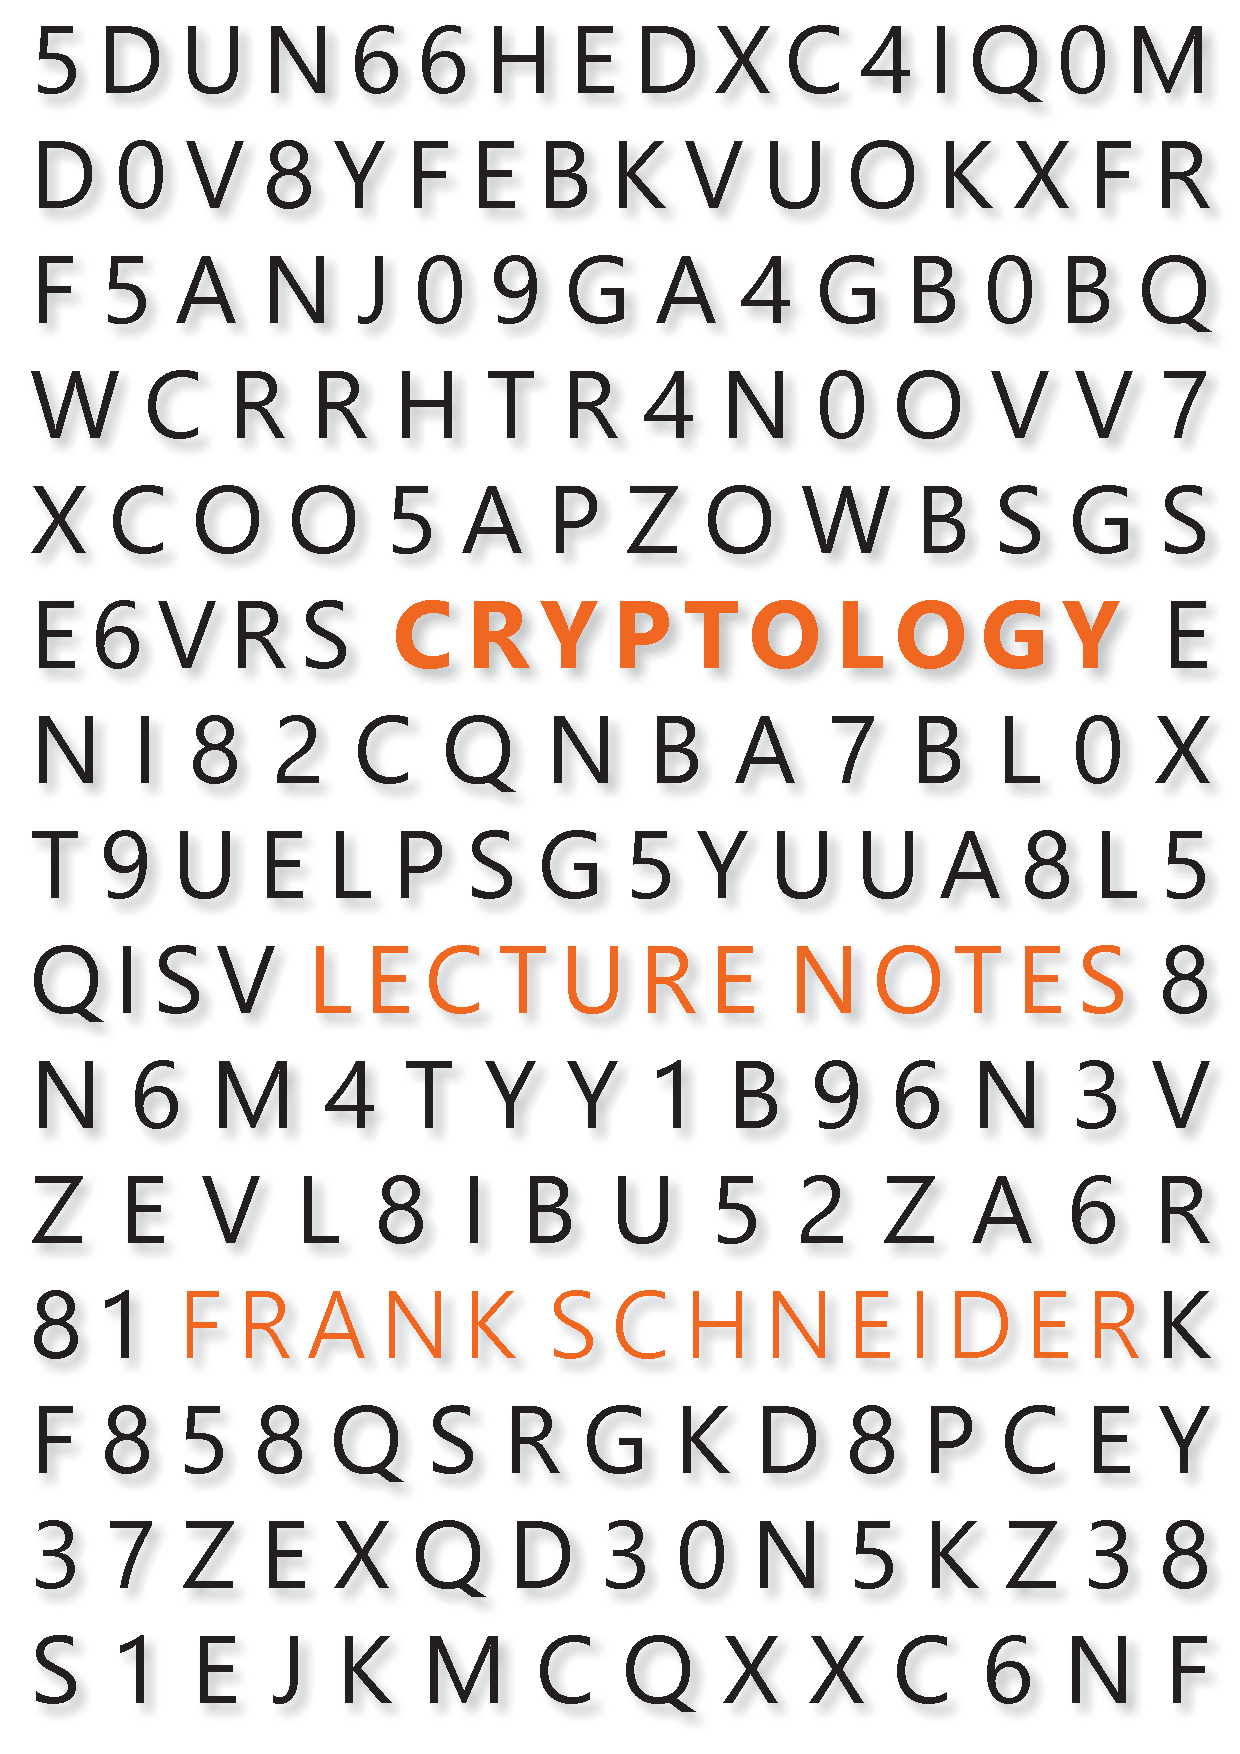
\includegraphics[width=0.99\paperwidth]{background2}}; % Background image
%\draw[anchor=north] (midpoint) node [fill=ocre!30!white,fill opacity=0.6,text opacity=1,inner sep=1cm]{\Huge\centering\bfseries\sffamily\parbox[c][][t]{\paperwidth}{\centering Cryptology\\[15pt] % Book title
%{\Large Lecture Notes 2015}\\[20pt] % Subtitle
%{\large by Frank Schneider}}}; % Author name
\end{tikzpicture}};
\end{tikzpicture}
\vfill
\endgroup

%----------------------------------------------------------------------------------------
%	COPYRIGHT PAGE
%----------------------------------------------------------------------------------------

\newpage
~\vfill
\thispagestyle{empty}

\noindent Copyright \copyright\ 2015 Frank Schneider\\% Copyright notice

\noindent This file was created as an inofficial transcript of the lecture ``Cryptology'' by \textsc{Tanja Lange} at the \textsc{Technische Universiteit Eindhoven} TU/e.\\

\noindent These lecture notes are only meant for personal use.\\

\noindent The figures used in this file are self-provided (adapted from the original lecture notes by \textsc{Tanja Lange} and \textsc{Ruben Niederhagen}) if not attributed otherwise. \\ 

\textit{\today} % Printing/edition date

%----------------------------------------------------------------------------------------
%	TABLE OF CONTENTS
%----------------------------------------------------------------------------------------

\chapterimage{Pictures/Header/Header.pdf} % Table of contents heading image

\pagestyle{empty} % No headers

\tableofcontents % Print the table of contents itself

\cleardoublepage % Forces the first chapter to start on an odd page so it's on the right

\pagestyle{fancy} % Print headers again


%----------------------------------------------------------------------------------------
%	CHAPTERS
%----------------------------------------------------------------------------------------

\chapter{Introduction}

\section{Cryptography vs. Cryptoanalysis}

Cryptography\index{Crypthography}: The constructive part (e.g. building systems, ``constructing the encryption''). \\
Cryptanalysis\index{Cryptanalysis}: The destructive part (e.g. breaking systems, ``cracking the code''). \\

This course covers both parts of Cryptology\index{Cryptology}. Both parts are needed in deployed systems, since we want to know how efficient the system is \textbf{and} how hard it is to break it:

\begin{example}
\ \\
\begin{itemize}
\item $2^{60}$ is inconvenient to compute, but totally doable;
\item $2^{70}$ is doable for academic clusters;
\item $2^{80}$ is doable for the NSA;
\item $2^{128}$ nobody can do that (including a security margin);
\end{itemize}
\end{example}

\begin{remark}
These numbers depend on the model of computation. Algorithms for example have different runtimes on quantum computers.
\end{remark}

%------------------------------------------------

\section{Caesar Cipher}\index{Caesar Cipher}

A standard example in cryptology is a \textsc{Caesar cipher}. In this example \textsc{Alice} (denoted \textsc{A} in figure \ref{fig:caesar_cipher}) wants to transmit a secret message ($E(m)$) to \textsc{Bob} (\textsc{B}), since the eavesdropper \textsc{Eve} (\textsc{E}) can see or hear everything on the channel.

\begin{figure}[H]
  \centering\import{Chapter1/Pictures/}{caesar_cipher.pdf_tex}
  \caption{Encrypted communication}
  \label{fig:caesar_cipher}
\end{figure}

So \textsc{Alice} and \textsc{Bob} decide to use a simple form of encryption - the \textsc{Caesars Cipher}. They replace the letters of the message by a letter some fixed number (in this case it is 3) of positions down the alphabet (see figure \ref{fig:caesar_cipher_ill}).

\begin{figure}[h]
\centering\includegraphics[scale=0.4]{Chapter1/Pictures/caesar_cipher_ill}
\caption{Idea of \textsc{Caesars Cipher}}
\label{fig:caesar_cipher_ill}
\end{figure}

\begin{example}
\ \\
The (original) message \\
 \textsc{HELLO} (Plaintext), 
 would be encrypted into \\
 \textsc{KHOOR} (Ciphertext)
\end{example}

This method of encryption is easy to cryptanalyze.

It is possible to turn this into a keyed encryption\index{Keyed Encryption}: $E_k(m)$, where the key $k$ gives the shifting distance. The decryption therefore is: $D_k(c)$, which should satisfy
\[
D_k(E_k(m)) = m.
\]

%------------------------------------------------

\section{Two types of crypto systems}

There are two types of crypto systems: \emph{symmetric} and \emph{asymmetric} (= public key) systems. In the \emph{symmetric} crypto \textsc{A} and \textsc{B} share the same key (e.g. the shifting distance of the \textsc{Caesars Cipher}, 128 bits in \textsc{AES}).

In \emph{public key} crypto each user has 2 keys:

\begin{itemize}
\item A \emph{public}\index{Public Key} one which can be used by anybody to encrypt messages to this user and
\item A \emph{private} (= secret key\index{Private Key}) one which the user uses to decrypt messages.
\end{itemize}

Therefore in \emph{asymmetric} systems this means $c= E_{P_k} (m), D_{S_k}(c) = m$, with $P_k$ the \emph{public key} and $S_k$ the \emph{secret key}. $P_k$ and $S_k$ can be of very different nature.

In a good crypto system one should not be able to recover $S_k$ from $P_k$ (= \emph{complete break}) or to decrypt $c$ without knowing $S_k$.

\begin{remark}
This means that there are two possiblities of cryptanalyzing a system. One can either find the \emph{secret key} or find the message. Obviously the first case means a \emph{complete break}, meaning that every other message can be decrypted as well.
\end{remark}

We will see different crypto systems such as \textsc{RSA}, \textsc{Elliptic-Curve Cryptography (ECC)} and \textsc{McEliece encryption} including attacks on these. \\

\noindent Crypto is also about authentication, e.g. digital signatures.

%TODO include Example of bank - asymmetric encryption


\chapter{Mathematic Repetition}

\section{Modulus Calculation}

\begin{notation} \ \\
$\Z$: integers $\{\dots,-3,-2,-1,0,1,2,3,\dots\}$ \\
$\nicefrac{\Z}{n}$: residue classes of $\Z$ modulo n \\
$\nicefrac{\Z}{6} = \{0,1,2,3,4,5\} = \{-2,-1,0,1,2,3\}$. \\
\end{notation}

We use integers to represent classes, so $0$ stands for the set of integers which are congruent to $0$ modulo $6$, i.e. $\{0,6,12,18,\dots,-6,-12,\dots\}$. You might have learned this as $\bar{0}$ to denote the class.

$7 \equiv 1 \bmod 6$ ($\widehat{=} 7$ is congruent to $1$ modulo $6$). Usually we want the small represantative on the right side; depends on set chosen, e.g. $17 \equiv 5 \equiv -1 \mod 6$.

\subsection{Multiplication}

If we have a multiplication with modulus n, e.g. $a \cdot b \bmod n$. We can compute the result and then reduce - or we could reduce at any intermediate step. $17 \cdot 35 \equiv -1 \cdot (-1) \equiv 1 \bmod 6$.

\subsection{Exponentiation}

If we want to compute an exponentiation with modulus n: $a^b \bmod n$, we write $b$ in binary:

\[
b = \sum\limits_{i=0}^{l-1} b_i 2^i;\,\, b_i \in \{0,1\} \,\, \text{ with } \,\, b_{l-1} = 1
\]

\begin{example} \ \\
$17 = 1 \cdot 2^4 + 0 \cdot 2^3 + 0 \cdot 2^2 + 0 \cdot 2^1 + 1 \cdot 2^0;$ \\ 
$35 = 1 \cdot 2^5 + 1 \cdot 2^1 + 1 \cdot 2^0$.
\end{example}

$a^b = a^{\sum b_i \cdot 2^i} = \Big( \dots \big( \big( a^{b_{l-1}2 + b_{l-2}}\big)^{2+b_{l-3}} \Big)^{2+\dots+2+b_0}$

\subsubsection{Square and Multiply}\index{Square and Multiply}

\begin{algorithm}[H]
$c \leftarrow a$ \;
 \For{$i = l-2$ down to $0$}{
 $c \leftarrow c^2 \bmod n$ \;
 \If{$b_i = 1$}{
 $c \leftarrow c \cdot a \bmod n$ \;
 }
 output $c$\;
 }
 \caption{Square and Multiply - pseudocode}
\end{algorithm}

\begin{remark}
This algorithm reduces at every intermediate step, making the exponentiation a lot simpler and faster.
\end{remark}

\subsection{Inverses}

Sometimes we need to calculate inverses, e.g. divide equation $\bmod 7$ by $4$, this means undo a multiplication by $4$. What we are looking for is to find an integer $a \bmod 7$, such that $4 \cdot a \equiv 1 \bmod 7$, other notation $a^{-1} \equiv 4 \bmod 7$.

Here $a \equiv 2 \bmod 7$ because $4 \cdot 2 \equiv 8 \equiv 1 \bmod 7$.

In general, use \textsc{Euclidean algorithm}\index{Euclidean Algorithm} to compute $a$.

\begin{remark}
Look up \textsc{XGCD-extended Euclidean algorithm}. %TODO
\end{remark}

Inverses do not exist if the numbers are not coprime, e.g. $4$ is not inversible $\bmod 6$.

\begin{notation}
Set of invertible integers $\bmod n$ is denoted by $(\nicefrac{\Z}{n})^{\ast}$
\end{notation}

\begin{example} \ \\
\begin{itemize}
\item $(\nicefrac{\Z}{7})^{\ast} =\{1,2,3,4,5,6\}$ with inverses $1^{-1} \equiv 1 \bmod 7$, $2^{-1} \equiv 4 \bmod 7$, $3^{-1} \equiv 5 \bmod 7$, $6^{-1} \equiv  6 \bmod 7$; these are exactly the integers coprime with $7$.
\item $(\nicefrac{\Z}{6})^{\ast} = \{1,5\}$
\item $(\nicefrac{\Z}{6})^{\ast} = \{1,2,3,\dots,p-1\}$ for $p$ prime.
\end{itemize}
\end{example}

\textsc{Euler's phi function} gives the size of $|(\nicefrac{\Z}{6})^{\ast}| = \varphi(n)$.

\begin{example}\ \\
\begin{itemize}
\item $\varphi(7) = 6$
\item $\varphi(6) = 2$
\item $\varphi(p) = p-1$
\end{itemize}
\end{example}

For the multiplication of two primes $p, q$ ($p \neq q$) you can calculate the \textsc{phi function} as follows:

\[
	\begin{matrix}
  \tikzmark{top}{0} & 1 & 2 & 3 & 4 & \dots & q-1 \\
  q & q+1 & q+2 & q+3 & \dots & & 2q-1 \\
  2q & \dots & & & & & \\
  \vdots & & & & & & \vdots \\
  \tikzmark{bottom}{(p-1)q} &  &  &  &  & & p \cdot q-1 \\
 \end{matrix}
 \DrawLine[ocre, thick, opacity = 0.7]{top}{bottom}
\]


The numbers in the first column are all divisible by $q$ (there are $p$ of them). They can be removed (since $p$ and $q$ are primes, this means that only numbers which are multiples of $p$ or $q$ are not coprime).

Do the same with $p$:
\[
\begin{matrix}
	0 & 1 & 2 & \dots & p-1 \\
\end{matrix}
\]
this removes $q$ values,
\[
\varphi(p \cdot q) = p \cdot q - p - q + 1
\]
\marginnote{Since the $0$ is removed twice, we have to add $+1$.}[-1cm]

\begin{example} \ \\
\begin{itemize}
\item $\varphi (2 \cdot 3) = 2 \cdot 3 - 2 - 3 + 1 = 2$ (same)
\item $\varphi (p^2) = p^2 - p$, in general:
\item $\varphi (p^b) = p^b - p^{b-1}$
\item if you have: $n = \prod\limits_{i=0}^{l-1} p_i^{e^i}$, $p_i \neq p_j$ then ($e_i \in \N \leq 1$)
\[
\varphi(n) = \prod(p_i^{e_i} - p_i^{e_i - 1})
\]
Test: $\varphi(p \cdot q) = (p-1)(q-1) = p \cdot q - p - q + 1$ as above.
\end{itemize}
\end{example}

\section{Lagrange's Theorem}

\begin{theorem}[Lagrange's Theorem]\index{Lagrange's Theorem}
Let $G$ be a finite group of size $|G| = l$ then for any $a \in G$ we have
\[
a^l = 1,
\]
where $1$ is the neutral element and $G$ is written multiplicatively
\end{theorem}

\begin{example}
$a^6 \equiv 1 \bmod 7$ for $a \in (\nicefrac{\Z}{7})^{\ast}$
\end{example}
\chapter{RSA}

The name \textsc{RSA}\index{RSA} comes from the initials of \textsc{Rivest}, \textsc{Shamir}, \textsc{Ademan}. In 1977 it was the first encryption and signature system with a public key.

\section{Generating the Keys}

We pick two large primes $p \neq q$, put $n=p \cdot q$ and compute $\varphi(n) = (p-1)(q-1)$.

Now pick an integer $e$, which is coprime with $\varphi(n)$.

Compute $e^{-1} \equiv d \bmod \varphi(n)$ using \textsc{XGCD}. \\

RSA public key: ($e,n$)
private key: d

\begin{example} \ \\
$p = 5$, $q = 7$, \\
$n = 5 \cdot 7 = 35$ \\
$\varphi(n) = (5-1)(7-1)=24$ \\
\begin{itemize}
\item Pick $e=5$, $gcd(5,24) = 1$, \\
$5^{-1} \equiv 5 \bmod 24$, so $d= 5$
\item Other options, e.g. $e = 7$. Compute $gcd$:
\[
\begin{matrix}
24 & 1 &0 & \\
7 & 0 & 1& q=3 \\
3 & 1 & -3 & q=2 \\
1 & -2 & 7& \\
\textcolor{ocre}r\textcolor{ocre}\uparrow \  & \textcolor{ocre}a\textcolor{ocre}\uparrow \  & \textcolor{ocre}b\textcolor{ocre}\uparrow \  & \\
\end{matrix}
\]
For every row, $q$ is the number of times the first item in the row ``fits into'' the item above it. So for $24$ and $e=7$ this means: $q= 34$ (since $7 \cdot 3 = 21$ with rest $3$). You then subtract 3 times this row from the previous row, or more general: subtract q times row from previous.

Every row now satisfies that $r = a \cdot 24 + b\ \cdot 7$, e.g. $1 = -2 \cdot 24 + 7 \cdot 7 \Rightarrow 7^{-1} \equiv 7 \bmod 24$
\end{itemize}
Then ($5,35$) public key and $d=5$ secret key or
($7,35$) public key and $d=7$ secret key.
\begin{remark}
It is pure coincidence (and due to the fact that we use small numbers) that $d$ and $e$ are equivalent)
\end{remark}
\end{example}

\section{Encryption and Decryption of message}

\subsection{Encryption}
We want to encrypt the message $m < n, m \in \N$.
\[
c \equiv m^e \bmod n
\]
\begin{remark}
At this point in an implementation we would use the Square and Multiply method.
\end{remark}

\subsection{Decryption}
To decrypt of c, we calculate:
\[
m' \equiv c^d \bmod n
\]
\begin{remark}
We now want to proof that the decryption undos the encryption, or as we stated earlier $D(E(m)) = m$, or in this case $m' = m$
\end{remark}
This decryption works because
\[
m' \equiv c^d \equiv (m^e)^d \equiv m^{e \cdot d} \equiv m^{1+k \varphi(n)} \equiv m \bmod n
\]

where $e \cdot d = 1 \bmod \varphi(n)$, i.e. $e \cdot d = 1 + k \cdot \varphi(n)$ for some $k$. 

For the last step, we used \textsc{Lagrange} with group $(\nicefrac{\Z}{n})^{\ast}$ because there $m^{\varphi(n)} \equiv 1 \bmod n$. You can check that $m^{1+k \varphi(n)} \equiv m \bmod n$ even when $gcd(m,n) \neq 1$. \\

To show this, use the \textsc{Chinese Remainder Theorem (CRT)}\index{Chinese Remainder Theorem}
\[ m \equiv 0 \bmod p \\
m \equiv a \bmod q, \,\, a \neq 0, \text{ then} \\
m^{e \cdot d} \equiv 0^{e \cdot d} \equiv 0 \bmod p
\]

In $(\nicefrac{\Z}{q})^{\ast}$ we have $a^{q-1} \equiv 1 \bmod q$.

Thus

\begin{align}
	m^{e \cdot d} \equiv a^{e \cdot d} &\equiv a^{1+k \varphi(n)} \equiv a^{1 + (p-1)(q-1)} \equiv a \cdot \big( \underbrace{a^{q-1}}_{=1}\big)^{p-1} \equiv a \cdot 1^{p-1} \equiv a \bmod q  \notag \\
	m^{e \cdot d} &\equiv 0 \equiv m \bmod p \notag \\
	m^{e \cdot d} &\equiv a \equiv m \bmod q, \notag
\end{align}

thus \textsc{CRT} gives $m^{e \cdot d} \equiv m \bmod n$.

Last case $0^{e \cdot d} \equiv 0 \bmod d \Rightarrow \text{ \textsc{RSA} gives } m' = m$.

\section{Making the Algorithm Faster}

To get a faster encryption, we can use a small $e$ when generating the key.

Choosing small $d$ gives \textsc{Eve} your key; but we can decrypt faster using \textsc{RSA-CRT}: Compute
\[
c^d \equiv m_p \bmod p \\
c^d \equiv m_q \bmod q \\
\]

This is faster because the operands are smaller (naivley this save a factor of $4$ in each computation, do this twice, so save factor of $2$).

Combine $m_p$ and $m_q$ using \textsc{CRT} to get $m$. \\

We can save more effort by noticing that $c^{p-1} \equiv \bmod p$, so compute $d_p \equiv d \bmod p-1$ and $d_q \equiv d \bmod q-1$; $d_p$ and $d_q$ have half the bit length of $d$, so the \textsc{Square and Multiply} loop is half as long in computing
\[
c^{d_p} \equiv m_p \bmod p \\
c^{d_q} \equiv m_q \bmod q \\
\]

Combine $m_p$ and $m_q$ to $m$ using \textsc{CRT}. This needs just one multiplication given $u \equiv p^{-1} \bmod q$ as precomputed value.

Then $m = m_p q \cdot v + p \cdot u \cdot m_q$ with $v \equiv q^{-1} \bmod p$. ``Naively'' because with \textsc{Karatsuba}, doublelength costs only 3 times as much and for very long integers the \textsc{Fast Fourier Transformation (FFT)}\index{Fast Fourier Transformation} takes only twice as long.
\chapter{Finite Fields}\index{Finite Field}

\begin{definition}[Fields]
A set $K$ is a \emph{field} with respect to $\circ$ and $\diamond$, denoted $(K, \circ, \diamond)$, if
\begin{enumerate}[label=\roman*]
\item $(K,\circ)$ is an abelian group:\index{Abelian Group}
\begin{itemize}
\item \textbf{closure} for all $a, b \in K \Rightarrow a \circ b \in K$
\item \textbf{associativity} $(a \circ b) \circ c = a \circ (b \circ c) \,\,\,\, a,b,c \in K$
\item \textbf{identity} there is a $e_0 \in K$ such that for all $a \in K$, $a \circ e_0 = e_0 \circ a = a$
\item \textbf{inverse} for all $a \in K$, there is a $b \in K$, such that $a \circ b = e_0$
\item \textbf{commutive} $a \circ b = b \circ a$
\end{itemize}
\item $(K^{\ast} =K \ \{e_0\}, \diamond)$ is an abelian group
\item the distributive law holds in $K$:
\begin{itemize}
\item[] $a \diamond (b \circ c) = a \diamond b \circ a \diamond c$
\end{itemize}
\end{enumerate}
\end{definition}

\begin{example} \ \\
\begin{itemize}
\item $(\N, +, \cdot)$ is \textbf{NOT} a finite field (e.g. there is no inverse for $+$)
\item $(\Z, +, \cdot)$ is \textbf{NOT} a finite field (e.g. there is no inverse for $\cdot$)
\item $(\Q, +, \cdot)$ is a finite field
\item $(\R, +, \cdot)$ is a finite field
\item $(\C, +, \cdot)$ is a finite field
\item $K = \{0,1\}$ is the smallest set we can get: \\

\bgroup
\def\arraystretch{1.5}
\begin{tabular}{c|cc}
$+$ &  0 & 1 \\
\hline 
0 & 0 & 1  \\
1 & 1 & 0 \\
\end{tabular} \hfill
\begin{tabular}{c|cc}
$\cdot$ &  0 & 1 \\
\hline 
0 & 0 & 0  \\
1 & 0 & 1 \\
\end{tabular} \hfill
relating to: \hfill
\begin{tabular}{c|cc}
$\circ$ &  $e_{\circ}$ & $e_{\diamond}$ \\
\hline 
$e_{\circ}$ & $e_{\circ}$ & $e_{\diamond}$  \\
$e_{\circ}$ & $e_{\diamond}$ & $e_{\circ}$ \\
\end{tabular} \hfill
\begin{tabular}{c|cc}
$\diamond$ &  $e_{\circ}$ & $e_{\diamond}$ \\
\hline 
$e_{\circ}$ & $e_{\circ}$ & $e_{\circ}$  \\
$e_{\diamond}$ & $e_{\circ}$ & $e_{\diamond}$ \\
\end{tabular}
\egroup \\ \\
The $+$ corresponds to \textsc{XOR}, the $\cdot$ to \textsc{AND}
\end{itemize}
\end{example}

\begin{definition}[Subfield]\index{Subfield}
If $(K, \circ, \diamond)$ and $(L,\circ, \diamond)$ are field and $K \subseteq L$ then $K$ is a \emph{subfield} of $L$.
\end{definition}

\begin{remark}
$\Rightarrow$ We can add elements of $L$ to and multiply them with elements of $K$ $\Rightarrow$ $L$ is a vectorspace over $K$ (other properties work because of the distributive laws.
\end{remark}

\begin{definition}[Extension Degree]\index{Extension Degree}
Let $L$ be a field and let $K$ be a subfield of $L$. The \emph{extension degree} $[L:K]$ is defined as $\dim_k L$, the dimension of $L$ as a $K$ vectorspace. 
\end{definition}

\begin{definition}[Characteristic]\index{Characteristic}
Let $K$ be a field. The \emph{characteristic} of $K$, denoted $\op{char}(K)$, is the smallest positive integer $m$ such that $\underbrace{e_{\diamond} \circ e_{\diamond} \circ \dots \circ e_{\diamond}}_{\makebox[0pt]{$\scriptsize\begin{array}{c}m \text{ copies of } e_{\diamond} \text{ denoted as } [m]e_{\diamond}\end{array}$}} = e_{\circ}$; if no such integer exists, $\op{char}(K) = 0$.
\end{definition}

\begin{lemma} \label{lemma:field}
The characteristic of a field is $0$ or a prime
\begin{proof}
Let $\op{char}(K) = n = a \cdot b \,\,\,\, 1<a,b<n$. Then
\[
	e_{\circ} = [m]e_{\diamond} = [a \cdot b]e_{\diamond} = [a]e_{\diamond} \diamond [b]e_{\diamond}
\]
Since a field has no zero divisors it must be that $[a]e_{\diamond} = e_{\circ}$ or $[b]e_{\diamond} = e_{\circ} \,\, \lightning$ to minimality of $\op{char}(K) = n$.
\end{proof}
\end{lemma}

\begin{remark}
In the proof of Lemma \ref{lemma:field} we repeatedly used the distributive law:
\begin{align*}
&[a]e_{\diamond} \diamond [b]e_{\diamond} \\
\iff &(e_{\diamond} \circ [a-1]e_{\diamond}) \diamond [b]e_{\diamond} 
\iff \underbrace{e_{\diamond} \diamond [b]e_{\diamond}}_{\makebox[0pt]{$\scriptsize\begin{array}{c}= [b]e_{\diamond}, \\ \text{ since }e_{\diamond} \text{ is the neutral} \\ \text{ element for } \diamond \end{array}$}} \circ [a-1]e_{\diamond} \diamond [b]e_{\diamond} \\
\iff &[b]e_{\diamond} \circ (e_{\diamond} \circ [a-2]e_{\diamond}) \diamond [b]e_{\diamond} 
\iff \dots \iff \underbrace{[b]e_{\diamond} \circ [b]e_{\diamond} \dots \circ [b]e_{\diamond}}_{a \text{ times } \,\, \rightarrow \,\, [a \cdot b]e_{\diamond}}
\end{align*}
\end{remark}

\begin{lemma}
A finite field $K$ has characteristic $p$ for some prime $p$
\begin{proof}
Since $K$ is finite, there must be $i,j \in \N$ with $[i]e_{\diamond} = [j]e_{\diamond}$. Let $i > j$ then $[i-j]e_{\diamond} = e_{\circ}$ and so $\op{char}(K)|(i-j)$.
\end{proof}
\end{lemma}

Let $K$ be a finite field. We will now explore its structure. We know already: $\ch(K) = p$ for a prime $p$, and there exists $e_{\circ}, e_{\diamond} \in K$ with $e_{\circ} \neq e_{\diamond}$. Since $K$ is closed under $\circ$ we do also find $[2]\ed, [3]\ed,\dots,[p-1]\ed,[p]\ed = \ec, [p+1]\ed = \ed, \dots$ a cyclic subgroup of order $p$ of $(K,\circ)$. Multiplying two such elements $[i]\ed \diamond [j]\ed = [ij]\ed$ again gives us an element of the set$\{[i]\ed | 0 \leq i < p\}$. The scalars are considered modulo $p$ because $[p]\ed = \ec$. Since $p$ is a prime, $i \cdot j \not \equiv 0 \bmod p$ for $0 < i,j < p$. This means that  $\{[i]\ed | 0<i<p\}$ forms a subgroup of $K^{\ast}$ (the multiplicative group in $K$; $K^{\ast} = K \backslash \{\ec\})$.

\begin{figure}[H]
  \centering\import{Chapter4/Pictures/}{ring_structure.pdf_tex}
  \label{fig:ring_structure}
\end{figure}

If two structures (groups, rings, fields,...) behave exactly the same way so that one can give a one-to-one map between them, mathematicians call these twostructures \emph{isomorphic}\index{Isomorphism}. Out considerations have found a subfield of $K$ which is isomorphic to $\nicefrac{\Z}{p \Z}$ with map $[i]\ed \longmapsto i + p \Z$.

\begin{definition}[Prime Field]\index{Prime Field}
Let $K$ be a field. The smallest subfield contained in $K$ is called the \emph{prime field} of $K$.
\end{definition}

\begin{lemma}
Let $K$ be a finite field of $\ch(K) = p$.\\
The prime field of $K$ is isomorphic to $\nicefrac{\Z}{p \Z}$
\begin{align*}
\ec &\longmapsto 0 & \text{ in } \nicefrac{\Z}{p \Z} \\
\ed &\longmapsto 1 & \text{ in } \nicefrac{\Z}{p \Z}
\end{align*}
\end{lemma}

Above we found that an extension field can be considered as a vectorspace over its subfield. From now on we identify the prime field of a finite field with $\nicefrac{\Z}{p \Z}$ and write $0$ for $\ec$ and $1$ for $\ed$. Let $[K:\nicefrac{\Z}{p \Z}] = n$, i.e., the dimension of $K$ as a vectorspace over $\nicefrac{\Z}{p \Z}$ is $n$. This means that there exists a basis of $n$ linearly independent ``vectors'' $\alpha_1,\alpha_2,\dots,\alpha_n$. This being a basis means that every element in $K$ can be written in a unique way as $\sum\limits_{i=1}^n c_i \alpha_i$ with $c_i \in \nicefrac{\Z}{p \Z}$. The $p^n$ different choices for $(c_1,c_2,\dots,c_n) \in \nicefrac{\Z}{p \Z}^n$ mean that $K$ has $p^n$ elements.

\begin{lemma}
Let $K$ be a finite field. There exists a prime $p$ and an integer $n \in \N_{>0}$ such that $|K| = p^n$ and $\ch(K) = p$.
\end{lemma}

\begin{notation}
A field of characteristic $p$ and dimension $n$ is $\F_{p^n}$ or $GF(p^n)$ (for ``\textsc{Galois} field'')\index{Galois Field}
\end{notation}

This implies that every finite field has a prime power as its cardinality, so in particular there are no fields of size $6, 10, 14, 15$ etc.

In this representation it is very easy to add elements:
\[
	\left(\sum\limits_{i=1}^n c_i \alpha_i \right) + \left(\sum\limits_{i=1}^n d_i \alpha_i \right) = \sum\limits_{i=1}^n \left(c_i+d_i\right) \alpha_i
\]
but for multiplying them we need to know $\alpha_i \cdot \alpha_j$ for $1 \leq i,j \leq n$.

\begin{remark}
From now on we write $+$ for the first operation $\circ$ and $\cdot$ for the second operation $\diamond$, since we see $K$ as an extension of $\nicefrac{\Z}{p\Z}$.
\end{remark}

Let's see whether we can find out more about the multiplicative strucure. Remember that for a group $G$ we have $[|G|]a = e$ for any $a \in G$ by the properties of the order of a group. Since $K$ is a field, $K^{\ast}$ is a group and it has one element, namely $0$, less than $K$; thus $|K^{\ast}| = p^n-1$.

\begin{lemma}
Let $K$ be a finite field. The multiplicative group $K^{\ast}$ is cyclic.
\end{lemma}

Thus, for every $a \in K^{\ast}$ we have $a^{p^n-1} = 1$.

Let's look at another field beyond $\nicefrac{\Z}{p \Z}$. We know that they must have $p^n$ elements for some $p$ and $n$ - so what about a field with $2^2 = 4$ elements? This should have a basis of size $2$, let's use $\alpha_i = 1$ and $\alpha_2 =a$ then $\F_4 = {0,1,a,a+1}$ and we can simply write out the addition table using the vectorspace structure: \\

\begin{tabular}{c|cccc}
$+$ &  $0$ & $1$ & $a$ & $a+1$ \\
\hline 
$0$ & $0$ & $1$ & $a$ & $a+1$  \\
$1$ & $1$ & $0$ & $a+1$ & $a$  \\
$a$ & $a$ & $a+1$ & $0$ & $1$  \\
$a+1$ & $a+1$ & $a$ & $1$ & $0$  \\
\end{tabular} \\

To write the multiplication table - if possible - we need to know what $a^2$ is in terms of $1, a$ and $a+1$. A table of a group has each element exactly once per row and column. So defining $a^2 = a$ conflict with having already entry $a$ in the first entry of this row (see left table below). Using $a^2 =1$ means that $a \cdot (a+1) = a^2 + a = 1 + a$ - but then the third column (in the middle table) has already $a+1$ in the first entry. Try $a^2 = a + 1$ then $a \cdot (a+1) = a^2 + a = (a+1) + a = 1$ and $(a+1) \cdot (a+1) = a^2 +a +a +1= a^2 +1 = (a+1)+1 = a$. \\

\begin{tabular}{c|ccc}
$\cdot$ &  $1$ & $a$ & $a+1$ \\
\hline 
$1$ & $1$ & $a$ & $a+1$  \\
$a$ & \hl{$a$} & \hl{$a$} &   \\
$a+1$ & $a+1$ &  &   \\
\end{tabular} \,\,
\begin{tabular}{c|ccc}
$\cdot$ & $1$ & $a$ & $a+1$ \\
\hline 
$1$ & $1$ & $a$ & \hl{$a+1$}  \\
$a$ & $a$ & $1$ & \hl{$a+1$}  \\
$a+1$ & $a+1$ &  &   \\
\end{tabular} \,\,
\begin{tabular}{c|ccc}
$\cdot$ &  $1$ & $a$ & $a+1$ \\
\hline 
$1$ & $1$ & $a$ & $a+1$  \\
$a$ & $a$ & $a+1$ & $1$  \\
$a+1$ & $a+1$ & $1$  & $a$  \\
\end{tabular} \\

The tables show all group properties except for associativity. We could probe this by checking all combinations but that is very cumbersome.

%TODO \F_8 ausschreiben, siehe Skript.

We could do the same that we just did with $\F_4$ now with $\F_8$, but this would take a while (we would now use $1, a$ and $b$ as a basis). The multiplication table is now $8 \times 8$. So the question arises: \\

\begin{problem}
How can we get this ``automatically''? How do we compute $\alpha_i \cdot \alpha_j$ without a lookup table?
\end{problem} 
\ \\
The idea is to use a polynomial ring to represent the field elements. A polynomial ring also spans a vector space - but contrast to the vector space, the multiplication of polynomials is well defined.

The polynomial ring\index{Polynomial Ring} over field $K$:
\[
	K[x] = \left\{\sum\limits_{i=1}^n a_i x^i | n \in \N, a_i \in K \right\}, \,\,\,\, f \in K[x], \,\, f = \sum f_i x_i.
\]
Let $n$ be the largest integer with $f_n \neq 0$ then $\deg(f) =n$, \emph{leading coefficient} $\op{LC}(f) = f_n$, \emph{leading term} $\op{LT} = f_x x^n$.

\begin{definition}[Irreducible]\index{Irreducible}
A polynomial $f \in K[x]$ is called \emph{irreducible} if $\deg(f) \geq 1$ and it cannot be written as a product of polynomials of lower degree over the same field, i.e. if $u|f$ then $u \in K$ or $u = f$ for all $u \in K[x]$ and $\deg(u) \leq \deg(f)$ \\
Otherwise $f$ is \emph{reducible}\index{Reducible}. Note that this depends on the field $K$.
\end{definition}

\begin{example} \ \\
\begin{itemize}
\item $x^2-1 = (x+1)(x-1)$ is reducible in $\R[x]$.
\item $x^4 + 2x +1 = (x^2 + 1)^2$ in $\R[x]$ has no roots but is reducible.
\item $x^2 +1$ is irreducible in $\R[x]$ but reducible in $\C[x]$ by $(x-i)(x+i)$.
\item $x^3+6x^2+4$ is irreducible in $\nicefrac{\Z}{7 \Z}$
\end{itemize}
\end{example}

We will now look again at $GF(8) = GF(2^3)$. The question arises, what is $a \cdot b$ or $a \cdot a^2 = a^3$ since $b= a \cdot a = a^2$? We chose $a^3 = a+1$ and then all operations followed by using this equality. This polynomial - $a^3 + a +1$ - does not factor over $GF(2)$. Other choices we considered, e.g. $a^3 + 1$ do in fact factor and it was exactly by considering these factors, e.g. $(a+1)$ and $(a^2 + a +1)$ that we derived contradictions, e.g. $(a+1)\cdot (a^2+a+1) = a^3+1 = 0$ (using $a^3=1$). In the end we worked in $GF(2)[a]/_{(a^3+a+1)GF(2)[a]}$ - the polynomial ring over $GF(2)$ modulo the irreducible polynomial $a^3+a+1$.

\begin{example}\ \\
We want to compute $a \cdot (a^2 + a) = a^3 + a^2$ and $(a+1) \cdot (a^2+a) = a^3 + \cancel{a^2} + \cancel{a^2} + a = a^3 +a$. For this we use the irreducible polynomial $a^3 + a +1$ and do a polynomial long division: \ \\

\bgroup
\def\arraystretch{1.5}
\begin{tabular}{clc}
\cline{2-2}
 \multicolumn{1}{r|}{$a^3 +a+1$} & $a^3+a^2$ & $ = 1$ \\
 & $a^3+a+1$ & \\
 \cline{2-2}
 & \multicolumn{1}{r}{$a^2+a+1$} & \\
\end{tabular}
\egroup \hfill
\bgroup
\def\arraystretch{1.5}
\begin{tabular}{clc}
\cline{2-2}
 \multicolumn{1}{r|}{$a^3 +a+1$} & $a^3+a$ & $ = 1$ \\
 & $a^3+a+1$ & \\
 \cline{2-2}
 & \multicolumn{1}{r}{$1$} & \\
\end{tabular}
\egroup

\end{example}

In general, this construction gives a finite field:
Let $f$ be an irreducible polynomial of degree $n$ over $GF(p)$. We define addition and multiplication on
\[
	GF(p)[x]/_{f(x)GF(p)[x]} = \left\{ \sum\limits_{i=0}^{n-1} a_i x^i | a_i \in GF(p) \right\}
\]
as addition and multiplication in $GF(p)[x]$ followed by reduction modulo $f(x)$. $\leadsto GF(p^n)$ \\ \\

Let $g \in GF(p^n)$, $f$ irreducible in $GF(p)$. $\op{gcd}(f,g) =1$ (The $\op{gcd}$ of $f$ and $g$ has to be $1$ since $f$ is irreducible) and \textsc{XGCD} computes polynomials $h$ and $l$ with
\begin{align*}
1 &= g \cdot h + f \cdot l \\
1 &\equiv g \cdot h \bmod f \\
h &\equiv g^{-1} \bmod f
\end{align*}

\begin{example} \ \\
The polynomial $f = x^3 + x^2 +1$ is irreducible over $GF(2)$. What is the inverse of $g = x^2 +1$ over $GF(2) \bmod f$? \\

\bgroup
\def\arraystretch{1.5}
\begin{tabular}{clc}
\cline{2-2}
 \multicolumn{1}{r|}{$x^2 +1$} & $x^3+x^2 +1$ & $ = x+1$ \\
 & \multicolumn{1}{r}{$-(x^3 + x)$} & \\
 \cline{2-2}
 & \multicolumn{1}{r}{$x^2+x+1$} & \\
 & \multicolumn{1}{r}{$-(x^2+1)$} & \\
 \cline{2-2}
 & \multicolumn{1}{r}{$x$}
\end{tabular}
\egroup \hfill

\[ \Rightarrow x^3 + x^2 +1= (x^2+1)(x+1)+x \qquad (\ast)\]

\bgroup
\def\arraystretch{1.5}
\begin{tabular}{clc}
\cline{2-2}
 \multicolumn{1}{r|}{$x$} & $x^2+1$ & $ = x$ \\
 & $-x^2$ & \\
 \cline{2-2}
 & \multicolumn{1}{r}{$1$} & \\
\end{tabular}
\egroup \hfill

\[ \Rightarrow x^2 +1=x \cdot x +1 \qquad (\ast \ast)\]
\begin{align*}
1 &= f \cdot ? + g \cdot ?
\end{align*}
\begin{align*}
1 &= (x^2+1) + x \cdot x  &\text{from } (\ast \ast)\\
&= (x^2 +1) + [(x^3+x^2+1)+(x^2+1)(x+1)]x & \text{from inserting } (\ast) \\
&= (x^2+1) + (x^3+x^2+1)x+(x^2+1)(x+1)x \\
&= (x^3+x^2+1)x+(x^2+1)+(x^+1)(x+1)x \\
&= (x^3+x^2+1)x+(x^2+1)[1+(x+1)x] \\
&= (x^3+x^2+1)x+(x^2+1)[x^2+x+1] \\
\end{align*}
\end{example}

\textbf{Alternative approach:}

We know that $a^{p^n} =a$ and $a^{p^2-1}=1$ for $a \in GF(p^n)$ (\textsc{Lagrange's} Theorem).

Thus $a \cdot a^{p^n-2} = a^{p^n-1} =1$.

So we can compute the inverse of $(x^2+1)$ as $x(^2+1)^6$ in $GF(8)$:

\[
	(x^2+1)^{8-2} = (x^2+1)^6 = (x^2+1)^4 \cdot (x^2+1)^2 = \large((x^2+1)^2\large)^2 \cdot (x^2+1)^2
\]

How do we find irreducible polynomials? We can pick a random polynomial and check if it is irreducible using ``\textsc{Rabin's} test of irreducibility''\index{Rabin's Test of Irreducibility}.

\begin{notation}
We denote $\F_q^{\ast}$ as  the multiplicative group of $\F_q$. $\F_q^{\ast} = \F_q \setminus \{0\}$ is a cyclic group and if $\F_q^{\ast} = \langle g \rangle$ then the generator $g$ is called a \emph{primitive element}.
\end{notation}

\begin{example}
\[
	\F_7^{\ast}: \,\, \langle 2 \rangle = \{2^0=1,2^1=2,2^2=4\}
\]
$2^3=1$, etc. so $\langle 2 \rangle$ contains only $3$ elements, so $2$ is not primitive.
\[
\langle 3 \rangle = \{1,3,2,6,4,5\} = \F_7^{\ast}
\]
so  $3$ is a primitive element.
\end{example}

\begin{lemma}
Let $G$ be a cyclic group of order $n$, then the order of any $a\in G$ satisfies:
\[
	\ord(a)|n
\]
\end{lemma}
\begin{remark}
$\ord(a)|n$ states how many times we need to multiply $a$ to receive $1$, i.\,e. $a^n=1$.
\end{remark}

\begin{example}\ \\
\begin{itemize}
\item $\ord(4) = 6$ in $\F_7^{\ast}$
\item $\ord(2) = 3$ in $\F_7^{\ast}$
\item $\ord(1) = 1$ in $\F_7^{\ast}$
\item $\ord(6) = 2$ in $\F_7^{\ast}$
\end{itemize}
\end{example}

\begin{lemma}
Let $G$ be a cyclic group of order $n$, let $\langle g \rangle = G$, and let $l|n$.
\[
\text{Then } \ord(g^{\nicefrac{n}{l}}) = l
\]
\begin{proof}
\[
1, g^{\nicefrac{n}{l}}, g^{2\nicefrac{n}{l}}, g^{3\nicefrac{n}{l}}, \dots, g^{l\nicefrac{n}{l}} = 1
\]
so $\ord(g^{\nicefrac{n}{l}})$ is no larger than $l$ and $i \cdot \nicefrac{n}{l}$ for $0 \leq i < n$ is less than $n$. Because $n$ is minimum for $g$, $l$ is minimal for $\nicefrac{n}{l}$.
\end{proof}
\end{lemma}

\begin{example}
\[
\langle 3 \rangle = \F_7^{\ast}; \,\, \ord(3^{\nicefrac{6}{2}} = 3^3) = \ord(6) = 2
\]
\end{example}

There are multiple elements of order $l$: all the $g^{i \cdot \nicefrac{n}{l}}$ have order dividing $l$ and if $gcd(i,l)=1$ then $\ord(g^{i \cdot \nicefrac{n}{l}}) = l$.

\begin{example}
\begin{align*}
&\F_{19}^{\ast} = \langle 2 \rangle \,\, , \,\, 19 - 1 = 18 = 2 \cdot 3^2 \\
&\{ 1,2,4,8,-3,-6,7,-5,9,-1,-2,-4,-8,3,6,-7,5,9 \} = \langle 2 \rangle \\
&2 \text{ has } \ord(6) \text{ , but } \ord(2^{2 \cdot \nicefrac{18}{6}}) = 3 \text{ , } \ord(2^{3 \cdot \nicefrac{18}{6}}) = 2
\end{align*}
This means there are $\varphi(l)$ elements of order $l$.
\end{example}
\chapter{Diffie-Hellman Key Exchange}\index{Diffie-Hellman Key Exchange}

\section{Introduction}

The \textsc{Diffie-Hellman Key Exchange} is used to secretly exchange keys for an encryption. The key exchange can be explained easily with an example:

\textsc{A(lice)} and \textsc{(B)ob} want to exchange a key, without letting the eavesdropper \textsc{E(ve)} know. Everybody (including) \textsc{Eve} knows a cyclic group $G$, a generator $g$ and its order $n$:

\begin{figure}[H]
  \centering\import{Chapter5/Pictures/}{DH.pdf_tex}
  \caption{Illustration of the\textsc{Diffie-Hellman key exchange}}{\textsc{A} and \textsc{B} both think of a number between $0$ and $n$ (this is $a$ and $b$ respectively). Now the compute $g^a$ and $g^b$ and exchange this information (so \textsc{Eve} knows $g^a$ and $g^b$. Then \textsc{A} computes $g^{b^a}$ and \textsc{B} computes $g^{a^b}$. So they both now know $g^{ab}$.}
  \label{fig:caesar_cipher}
\end{figure}

In summary, this means that \textsc{A} computes $h_b^a = (g^b)^a = g^{ba} = g^{ab}$ and \textsc{B} computes $h_a^b = (g^a)^b = g^{ab}$. So \textsc{A} and \textsc{B} both share $g^{ab}$, while Eve only knows $g$, $h_a = g^a$, $h_b =g^b$.

\section{Computational DH Problem (CDHP)}\index{Computational DH Problem (CDHP)}

Given $g$, $g^a$, $g^b$ compute $g^{ab}$.

In groups that are good for crypto there are no efficient attacks on the \textsc{CDHP}.

\begin{example} Examples for these ``good groups'' are:
\begin{itemize}
\item elliptic curves over finite fields
\item multipl. groups of finite fields
\end{itemize}
\end{example}

\section{Decisional DH Problem (DDHP)}\index{Decisional DH Problem (DDHP)}

Given $g$, $g^a$, $g^b$ and $g^c$.

Decide whether $g^c = g^{ab}$.

Proofs for protocols often use \textsc{DDHP} rathen than \textsc{CDHP}.

Bad groups would be: $\langle 2 \rangle \subseteq \Q^{\ast}$:
\[
1,2,4,18,16 \cdots, 2^i, \dots  \qquad \text{no reduction}
\]
$h_a=2^a$, \textsc{E} takes $\log$ and gets $a$.

\section{Discrete Logarithm Problem (DLP)}\index{Discrete Logarithm Problem}

Given $g$ and $g^a$, compute $a$.

Solving \textsc{DLP} implies solving \textsc{CDHP} implies solving \textsc{DDHP}. Usually \textsc{DLP} is the best attack we know on \textsc{DHP}, but there is no equivalence.

In browser \textsc{DH} or \textsc{DHE} indicates that \textsc{DH} in finite fields is used. 

\textsc{DH\textbf{E}}: ephemeral \textsc{DH}, i.\,e. use a new key for every connection or for each time interval.
Perfectly forward secrecy. Somebody taking over your system at time $t$ should not be able to decrypt any message prior to time $t$ (or $t-t_0$, where $t_0$ is the time for the ephemeral key).

\textsc{DH}: \textsc{Diffie-Hellman} with longterm keys.

Crypto parameters choose $p$ to have $\geq 2048$ bits and prime, work in $\F_p^{\ast}$, are okay with long-term use; ephemeral is to deal with stuff outside crypto.

\textsc{A(lice)} and \textsc{B(ob)} use share $g^{ab}$ after running it through a hash function to get a fixed-length string ($128$ or $256$ bits) with good distribution. Cryptographic hash functions are also:

\begin{itemize}
\item \emph{pre-image resistant},i.\,e. cannot find $g^{ab}$ from $h(g^{ab})$
\item \emph{second-pre-image resistant}, i.\,e. cannot find another pre-image given the first one
\item \emph{collision resistant}, i.\,e. cannot find two strings $m_1$ and $m_2$ with $h(m_1) = h(m_2)$.
\end{itemize}

\begin{remark}
We know that $m_1$ and $m_2$ exist, but we don't want to be able to compute them.
\end{remark}

In \textsc{DH} we use $h(g^{ab})$ as shared key in symmetric crypto, e.\,g. \textsc{AES}.

\section{ElGamal Encryption}\index{ElGamal Encryption}

General parameters: $g$, $n$

\textsc{Alice's} public key: $h_a = g^a$

\textsc{Alice's} secret key: $a$

Encryption: Pick random $0<k \leq n$, compute $r=g^k$, $c=h_a^k \cdot m$ (assume $m \in G$), with $m$ the message. We then send $(r,c)$.

Decryption: $\nicefrac{c}{r^a} = m'$. This works, i.\,e. $m=m'$ because
\[
	\frac{c}{r^a} = \frac{h_a^k \cdot m}{(g^k)^a} = \frac{\cancel{(g^a)^k} \cdot m}{\cancel{(g^a)^k}} = m
\]

In practice, \textsc{ElGamal} is not used like this because $m \not \in G$. Instead $c= AES_{h(h_a^k)}(m)$ and $m'$ is computed by first computing $K = h(r^a)$ and then $AES_K(c) = m'$. This corresponds to asymmetric \textsc{DH}.

\textsc{A} has longterm key, sender has $K$, $r$ as one time keys, but \textsc{DH} uses $h_a^K$ directly as key instead of transmitting $m$.

\subsection{ElGamal Signature Scheme}\index{ElGamal Signature Scheme}

Parameters as above; signature proves that the signer has access to $a$. Signature is on $h(m)$ not $m$ - fixed length; no algebraic relations.

\emph{Sign:} Pick \textbf{one-time} $0<k<n$ nonce (= number used only once), compute $r=g^k$, compute $s=k^{-1}(h(m) - a \cdot r) \bmod n$. The signature is $(r,s)$.

\emph{Verify:} Does $g^{h(m)}$ equal $h_a^r \cdot r^s$? A valid signature passes verification because:
\[
	h_a^r \cdot r^s = g^{ar} \cdot g^{k(k^{-1}(h(m) - ar))} = g^{h(m)} \qquad \surd
\]
Anybody knowing $a$ can sign. This becomes a problem if the $a$ being used, becomes known:

We see $(r,s)$ on $m$, so we can compute
\[
	s \cdot k = h(m) - a \cdot r \,\, \overset{\substack{\text{since } \\ s, k, r, h(m) \\ \text{ are known}}}{\implies} \,\, a = \frac{h(m) - s \cdot k}{r} \bmod n
\]

So we can recover \textsc{A}'s longterm secret $a$ with just one leaked nonce $k$.
We can also recover $a$ if $k$ is reused (see the homework), we can detect this from seeing repeated $r$.

\begin{remark}
The problem of re-using $k$, made the first \textsc{Playstation} open for attacks
\end{remark}

This means that \textsc{ElGamal} signatures are somewhat fragile. We can work around this by choosing $k$ pseudorandomly, i.\,e. \textsc{A} has two secrets: $a$ and $k_a$, compute $k$ as $k = h(k_a,m)$. This gives the same $k$ for repeated $m$, but the attack on repeated $k$ needs different $m$'s. If you want a shorter secret have a master secret key $s_a$ and derive $a=h(s_a, \alpha)$ - with $\alpha$ a string ``nonce key''.

Note that biases in $k$ also lead to breaks via the hidden number problem (we may take about this later), so would need really good randomness for each $k$ - or this construction.

Properties of hash functions are important here because a second pre-image of $h(m)$, i.\,e. a message $m'$ with $h(m) = h(m')$ can just use the same $(r,s)$.

If \textsc{E} has colliding messages $m_1$ and $m_2$, where $m_1$ is innocent, she can ask \textsc{A} to sign $m_1$ and use that $(r,s)$ as signature on $m_2$.

\section{Pohlig-Hellman Attack}\index{Pohlig-Hellman Attack}

For the \textsc{DDH} we know $g$, $g^a$, $g^b$, $g^c$, and the problem is, is $g^c = g^{ab}$?

Sometimes we can solve this without solving \textsc{CDH}:
\begin{align*}
&\F_{19}^{\ast} = \langle 2 \rangle  & h_a = 7, \qquad h_b = 11 \\
&g^c = 13 \overset{?}{=} DH(7,11) &
\end{align*}

We can figure out if $a$ was even or odd. $\ord(2) = 18$, so $18$ is smallest power of $2$ giving $1$. \\

If $a = 2a'$, then $h_a^9 = 2^{a 9} = 2^{2a' 9} = 2^{18a'} = 1$

else $a = 2a'+1$, then $h_a^9 = 2^{9(2a'+1)} = 2^{9} = 18$

$7^9 = 1$ same for $h_b$: $11^9 = 1$, so $a$ and $b$ are both even, so $a \cdot b$ is even.

Try $13^9$ to see whether it can be $2^{ab}: 13^9 = 18 \implies$ this is not $g^{ab} \implies$ we solved \textsc{DDH}.

This way we can solve the \textsc{DDH} whenever parity of $c$ and $ab$ does not match. \\

To make statements about probability of solving  \textsc{DDH} we work with sequences of triples and try to distinguish $(g^a, g^b,g^{ab})$ from $(g^a, g^b,g^c)$ with random $c$.

Avoid this \textsc{DDH} weakness by picking $g$ to have odd order, so in $\F_19^{\ast}$ use the subgroup generated by $2^2 = 4$ of order $9$. This doesn't solve all our problems, we can check whether $g^{ab}$ and $g^c$ match as third powers: \\

$7^{\nicefrac{18}{3}} = 7^6 = 1$ shows that $a$ is a multiple of $3$, thus $a \cdot b \equiv 0 \bmod 3$. Try whether $13$ matches this, here $13^6 = 11$, so another proof that $(7,11,13)$ is not a valid \textsc{DDH} triple. \\

Can we find out more about $a$ and $c$? We know:
\[
\left. \begin{array}{l} a \equiv 0 \bmod 2\\
a \equiv 0 \bmod 3  \end{array}\right\} a \equiv 0 \bmod 6 
\]

we also  know $0<a< 18$, i.\,e. $a=6$ or $a=12$. We can check the two possibilities and get $2^6 = 7$, so $a=6$.

\begin{remark}
This is sort of a ``brute-force'' approach.
\end{remark}

We know $c \equiv 1 \bmod 2$ and $c \not\equiv 0 \bmod 3$. So $c = c_0 + 3 \cdot c_1$, so $2^c = 2^{c_0 + 3 c_1}$, thus $2^{c \cdot 6} = 2^{6(c_0 + 3 c_1)} = 2^{6c_0}$ this gave $13^6=11$, so determine $c_0$, compare $11$ with $2^6$ (i.\,e. $c_0=1$) and $2^{12}$ (i.\,e. $c_0 = 2$).
\[
\text{Here: } 2^6 = 7 \qquad 2^{12} = 11 \qquad \implies \text{ so } c_0 = 2, c = 2 + 3 \cdot c_1
\]

With \textsc{CRT} we know $c \equiv 1 \bmod 2$ $c \equiv 2 \bmod 3$ $\implies c \equiv 5 \bmod 6$, so it could be $5$, $11$ or $17$.

We could just try these $3$ but we want a systematic way of computing \textsc{DL} in groups of composite orders.

\begin{align*}
&2^c = 2^{2+3 c_1} \qquad \text{ ,so} \\
&2^{3c_1} = \nicefrac{13}{4} = 8 \qquad \text{ , get } c_1 \text{ by computing} \\
&2^{3c_1 } =2^{6c_1} = 8^2 = 7 \qquad \text{ and then comparing to} \\
&2^0 = 1, 2^6 = 7 \text{ and } 2^{12}=11 \implies c_1=1
\end{align*}

$\implies$ complete set:
\[
c \equiv 1 \bmod 2 \\
c \equiv 5 \bmod 9 \\
\rightarrow c = 5
\]

This \emph{\textsc{Pohlig-Hellman} attack} solves the \textsc{DLP} in all subgroups of prime order and then combines the results using \textsc{CRT}.

\begin{example}\ \\
$\F_{37}^{\ast} = \langle 2 \rangle$, find $a = \log_2 17$,

the group has subgroups of order $2,3,4,9$ (and others of non-prime order)

\[
	17^{18} = 36 \implies a \equiv 1 \bmod 2
\]
\[
	17^{12} = 26, \text{ so } a \not\equiv 0 \bmod 3
\]

compare with $2^{12} = 26$ and with $2^{2 \cdot 12} = 10 \rightarrow a \equiv 1 \bmod 3$.

To get $a \bmod 4$, compute $(\nicefrac{17}{2})^9 = 27^9 = 36 \Rightarrow a \equiv 1 + 1 \cdot 2 \equiv 3 \bmod 4$.

Same for $\bmod 9$: $(\nicefrac{17}{2})^4 = 27^4 = 10 \implies a =1+2 \cdot 3 \equiv 7 \bmod 9 \implies a \equiv 7 \bmod 36$.

\end{example}
\chapter{Hash Functions}\index{Hash Functions}


\chapter{Elliptic Curves}\index{Elliptic Curves}

\subsubsection{Warm Up}

The clock: $x^2 + y^2 = 1$ (not elliptic)

\begin{tikzpicture}[scale=3.0,cap=round,>=latex]
        % draw the coordinates
        \draw[->] (-1.2cm,0cm) -- (1.2cm,0cm) node[right,fill=white] {$x$};
        \draw[->] (0cm,-1.2cm) -- (0cm,1.2cm) node[above,fill=white] {$y$};
		\coordinate (O) at (0,0);
		\coordinate (1200) at (0,1);
		\coordinate (0130) at ({sqrt(0.5)},{sqrt(0.5)});
		\coordinate (0200) at ({sqrt(0.75)},0.5);
		\coordinate (0330) at (0.96592,-0.258819);
        % draw the unit circle
        \draw[dotted] (0cm,0cm) circle(1cm);
        \draw[fill] (1,0) circle [radius=0.025];
        	\node [below right] at (1,0) {$1$};
        	\node [above right] at (1,0) {3:00 $\overset{\sim}{=}(1,0)$};
        \draw[fill] (0,1) circle [radius=0.025];
        	\node [below left] at (0,1) {$1$};
        	\node [above right] at (0,1) {12:00 $\overset{\sim}{=}(0,1)$};
		\draw[fill] (-1,0) circle [radius=0.025];
        	\node [below left] at (-1,0) {$-1$};
        	\node [above left] at (-1,0) {9:00 $\overset{\sim}{=}(-1,0)$};
        \draw[fill] (0,-1) circle [radius=0.025];
        	\node [below right] at (0,-1) {$-1$};
        	
        \draw[gray] (0,0) -- ({sqrt(0.5)},{sqrt(0.5)});
        \draw[fill] ({sqrt(0.5)},{sqrt(0.5)}) circle [radius=0.015];
        	\node [above right] at ({sqrt(0.5)},{sqrt(0.5)}) {1:30 $\overset{\sim}{=} 2x^2 = 1 \implies x = y = \sqrt{\nicefrac{1}{2}}$};
        \draw[fill] ({sqrt(0.75)},0.5) circle [radius=0.015];
        \draw[gray] (0,0) -- ({sqrt(0.75)},0.5);
        	\node [right] at ({sqrt(0.75)},0.5) {2:00 $\overset{\sim}{=} (\sqrt{\nicefrac{3}{4}},\nicefrac{1}{2})$};
		\draw[fill] (-0.5,{sqrt(0.75)}) circle [radius=0.015];
        	\node [left] at (-0.5,{sqrt(0.75)}) {11:00 $\overset{\sim}{=} (-\nicefrac{1}{2},\sqrt{\nicefrac{3}{4}})$};
        	\markangle[yellow]{1200}{O}{0200}{\small$\alpha_2$}{3};
        	\markangle[ocre]{1200}{O}{0130}{\small$\alpha_1$}{2};
        	\markangle[green]{1200}{O}{0330}{\small \qquad \qquad $\alpha_1 + \alpha_2$}{1};
        	\draw[gray] (0,0) -- (0330);
        	\draw[fill] (0330) circle [radius=0.015];
\end{tikzpicture}

We also have ``strange'' (= non clock) points, such as $(\nicefrac{3}{5},\nicefrac{4}{5})$.

Define addition of clock points: Add points by adding angles; this matches addition of areas, addition of arch length and addition of times (e.\,g. $1:30 + 2:00 = 3:30$).

\section{Trigonometric Formulas}\index{Trigonometric Formulas}

\begin{tikzpicture}[scale=3.0,cap=round,>=latex]
        % draw the coordinates
        \draw[->] (-0.5cm,0cm) -- (1.2cm,0cm) node[right,fill=white] {$x$};
        \draw[->] (0cm,-0.5cm) -- (0cm,1.2cm) node[above,fill=white] {$y$};
        
        \draw[scale=0.5,domain=0:1.8,smooth,variable=\x,black] plot ({\x},{\x});
        \draw[fill](0,1) (0,1) circle [radius=0.025];
        \node [left] at (0,1) {$1$};
        \draw [gray,dotted,domain=0:90] plot ({cos(\x)}, {sin(\x)});
        \coordinate (O) at (0,0);
        \coordinate (M) at ({sqrt(0.5)},{sqrt(0.5)});
        \markangle[ocre]{0,1}{O}{M}{\small$\alpha$}{3};
        
        \draw[-,ocre] (0,{sqrt(0.5)}) -- (M) node[above left,fill=white] {\small $x(\alpha) = \sin(\alpha)$};
        \draw[-,ocre] ({sqrt(0.5)},0) -- (M);
        \node[ocre, below right,fill=white] at ({sqrt(0.5)},0.5) {\small $y(\alpha)= \cos(\alpha)$};
\end{tikzpicture}

\begin{align*}
x(\alpha_1 + \alpha_2) &= \sin (\alpha_1 + \alpha_2) = \sin \alpha_1 \cos \alpha_2 + \sin \alpha_2 \cos \alpha_1 = x(\alpha_1) y(\alpha_2) + x(\alpha_2)y(\alpha_1) \\
y(\alpha_1) + \alpha_2) &= \cos (\alpha_1 + \alpha_2) = \cos \alpha_1 \cos \alpha_2 - \sin \alpha_1 \sin \alpha_2 = y(\alpha_1) y(\alpha_2) - x(\alpha_1)x(\alpha_2)
\end{align*}

Addition law:
\[
(x_1,y_1) + (x_2,y_2) = (x_1y_1+x_2y_1,y_1y_2-x_1x_2)
\]

No more angles, can use any $(x,y)$ on circle.

\begin{example}
\begin{align*}
&\left(\nicefrac{3}{5},\nicefrac{4}{5} \right) + \left(\nicefrac{3}{5},\nicefrac{4}{5} \right)= \left(2 \,\, \nicefrac{3}{5} \,\, \nicefrac{4}{5},\left(\nicefrac{4}{5}\right)^2 - \left(\nicefrac{3}{5}\right)^2\right) = \left(\nicefrac{24}{25},\nicefrac{7}{25} \right) = 2 \left(\nicefrac{3}{5},\nicefrac{4}{5} \right) \\
&\left(\nicefrac{3}{5},\nicefrac{4}{5} \right) + \left(\nicefrac{24}{5},\nicefrac{7}{5} \right)= \left(\nicefrac{117}{125},\nicefrac{-44}{125} \right) = 3 \cdot \left(\nicefrac{3}{5},\nicefrac{4}{5} \right) \\
&4 \cdot \left(\nicefrac{3}{5},\nicefrac{4}{5}\right) = \left(\nicefrac{336}{625},\nicefrac{-527}{625} \right) \dots
\end{align*}
\end{example}

These all lie on the curve (= circle), lots of points.

Does this addition match the clock? 
\[
\left(\nicefrac{3}{5},\nicefrac{4}{5} \right) + \underbrace{\left(0,1\right)}_{\mathclap{\text{12 o'clock, no change to first part?}}} = \left(\nicefrac{3}{5} \cdot 1 + 0 \cdot \nicefrac{4}{5},\nicefrac{4}{5} \cdot 1 - \nicefrac{3}{5} \cdot 0 \right) = \left(\nicefrac{3}{5},\nicefrac{4}{5} \right)
\]

In general
\[
\left(x,y \right) + \left(0,1\right) = \left(x \cdot 1 + 0 \cdot y, y\cdot 1 - x \cdot 0 \right) = \left(x,y \right) \implies \left(0,1\right) \text{ is the neutral element}
\]

Show that $\left(x_1,y_1\right) + \left(x_2,y_2\right)$ is on circle.

Associativity holds because $\alpha_1 + (\alpha_2 + \alpha_3) = (\alpha_1 + \alpha_2) + \alpha_3$ and the link $x=\sin \alpha$, $y=\cos \alpha$.

$-\left(x,y\right) = \left(-x,y\right)$ (matching $-\alpha$, or just test $\left(x,y\right) + \left(-x,y\right) = \left(xy - xy. y^2 - (-x^2)\right) = (0,\underbrace{x^2+y^2}_{\mathclap{=1 \text{ because we're on the circle}}}) = \left(0,1\right)$

$\implies$ group; also commutative: $\alpha_1 + \alpha_2 = \alpha_2 + \alpha_1$ 

\section{Using Finite Fields}

Can use the circle addition law for $\left(x,y\right) \in k^2$ for any field $k$ with $x^2+y^2 = 1$ (no divisions in the formulas, could even use a ring here). For cryptography don't use $k = \Q$, else $a \cdot \left(x,y\right)$ gives away easy information on  $a$, e.\,g. $a \cdot \left(\nicefrac{3}{5},\nicefrac{4}{5} \right) = \left(\nicefrac{\dots}{5^a},\nicefrac{\dots}{5^a} \right)$, instead use finite field $\F_q$; this ``wraps around'' so we don't get size information. ``Bad'' points for crypto:

\begin{itemize}
\item $\left(0,1\right)$ (neutral element, so $a \cdot \left(0,1\right) = \left(0,1\right)$)
\item $\left(0,-1\right)$ point of order $2$: $2a \cdot \left(0,-1\right) = \left(0,1\right), (2a+1) \left(0,-1\right) = \left(0,-1\right)$
\item $\left(\pm 1,0\right)$ have order $4$
\item $\left(x,x\right)$, i.\,e. $1:30$ and the other sign combinations have order $8$
\item other points of small finite order
\item Modulo $p$ there are no points of infinite order - there are at most $p^2$ candidate points and of these only $p-1$ or $p+1$ are on the circle. (Plug in $x$, check whether $1-x^2$ is a square, if so we've found two points: $(x,y), (x,-y)$).
\end{itemize}

\begin{example} \ \\
$p = 17$
\begin{align*}
&x=0: &1-0^2 =1 = (\pm 1)^2 \implies (0,\pm 1) \\
&x=1: &1-1^2 =0 = 0^2 \implies (1,0) 
\end{align*}
symmetry gives also $(-1,0)$
\begin{align*}
&x=\pm 2: &1-4 =-3 = 14 \bmod 17 = \square \,\, ?? 
\end{align*}

\bgroup
\def\arraystretch{1.5}
\begin{tabular}{c|c|c|c|c|c|c|c|c|c}
 $z$ & $0$ & $\pm1$ & $\pm2$& $\pm3$& $\pm4$& $\pm5$& $\pm6$& $\pm7$& $\pm8$ \\ \hline
$z^2$& $0$ & $1$ & $4$& $9$& $16$& $8$& $2$& $15$& $13$
\end{tabular}
\egroup \ \\

$\implies$ ``half'' of all numbers appear, clear becaus $\F_q^{\ast} = \g$, so $g^{2a}$ are squares, $g^{2a+1}$ are non squares, also 0 is a square $\implies$ half means $\nicefrac{p+1}{2}$; in $\F_{2^n}$ every element is a square.
$14$ is not in the table $\implies$ no point with $x= \pm 2$

\begin{align*}
&x=\pm 3: &1-9 =9 = (\pm 3)^2 \implies (\pm 3, \pm 3) \\
&x=\pm 4: &1-16 =2 = (\pm 6)^2 \implies (\pm 4, \pm 6)
\end{align*}

$\implies 4$ more points using symmetries $(\pm 6, \pm 4)$

\begin{align*}
&x=\pm 5: &1-25 =10 \neq \square \,\,\text{ no points} \\
&x=\pm 7: &1-49 =1-15 = 3  \neq \square \,\,\text{ no points} \\
&x=\pm 8: &\text{ by symmetry, only candidates are } (\pm 8, \pm 8): \\
& &\text{ test } 8^2+8^2 = -4-4 = -8 \neq 1 \implies \text{ no points}
\end{align*}
Set of all points: $\left\lbrace(0,\pm 1), (\pm 1,0), (\pm 3, \pm 3), (\pm 4, \pm 6), (\pm 6, \pm 4) \right\rbrace \implies 16 = 17 - 1$ points. Try $p=19$ yourself.

\begin{remark}
For the case $x=\pm 8$, we used symmetry. If $8$ would pair up with another point, say $(\pm 8 , \pm 3)$ then by symmetry the point $(\pm 3, \pm 8)$ would also work. Since this was not the case in any of the numbers before $8$, this means that $8$ can only ``pair'' with itself.
\end{remark}
\end{example}

For crypto choose $p$ large enough and so that a large prime order subgroup appears. Sadly enough index calculus attacks apply to the circle; this is just a complicated description of a subgroup of $(\F_p^2)^{\ast}$ (or $\F_p \times \F_p$ ?).

\section{Edwards Curves}\index{Edwards Curves}

Tweak circle equation to $x^2 + y^2 = 1 + dx^2y^2$ (avoid $d=0$ and $d=1$). This keeps all symmetries, so $(x,y) \implies (\pm x, \pm y)$ and $(\pm y, \pm x)$.

\begin{tikzpicture}[scale=2.7,cap=round,>=latex]
        % draw the coordinates
        \draw[->] (-1.2cm,0cm) -- (1.2cm,0cm) node[right,fill=white] {$x$};
        \draw[->] (0cm,-1.2cm) -- (0cm,1.2cm) node[above,fill=white] {$y$};
		\draw [gray,dotted,domain=0:90] plot ({cos(\x)}, {sin(\x)});
		\draw plot[id=curve, raw gnuplot] function{
      f(x,y) = (x**2 + y**2) - 1 -(x**2 * y**2)*-20;
      set xrange [-1:1];
      set yrange [-1:1];
      set view 0,0;
      set isosample 1000,1000;
	  set size square;
      set cont base;
      set cntrparam levels incre 0,0.1,0;
      unset surface;
      splot f(x,y)
    };
		\draw[fill] (0,1) circle [radius=0.015];
        	\node [above right] at (0,1) {$1$};
       	\draw[fill] (1,0) circle [radius=0.015];
        	\node [below right] at (1,0) {$1$};
        \coordinate (O) at (0,0);
        \coordinate (M) at ({sqrt(0.5)},{sqrt(0.5)});
       \draw[->] (M) -- (0.43,0.43);
\end{tikzpicture}

This looks like a 4-legged starfish.

We now want do define the addition $(x_1,y_1) + (x_2,y_2) = (x_3,y_3)$ with
\[
x_3 = \frac{(x_1y_2 + x_2y_1)}{(1+dx_1x_2y_1y_2)} \qquad y_3 = \frac{(y_1y_2-x_1x_2)}{(1-dx_1x_2y_1y_2)}
\]

if $x$ or $y = 0$ then same as on circle; $\implies$ $(0,1)$ is still the neutral element. 

We now can check the inverse element $-(x,y) = (-x,y)$ because:
\[
x_3 = \frac{(xy - xy)}{(1-dx^2y^2)} = 0 \,\,\,\, \textcolor{ocre}{\checkmark} \qquad y_3 = \frac{(y^2+x^2)}{(1+dx^2y^2)}
\]
on \textsc{Edwards curve} $x^2+y^2 = 1 +dx^2y^2$, the numerator and denominator are equal, so $y_3 = 1$ (giving us $(0,1)$ as a result, which is in fact the neutral element).

Use computer to verify that $(x_3,y_3)$ is on curve and that the addition is associative.

Attention: We have divisions here!!

Over $\R$ we can argue with sizes to see that $0 \leq |dx_1x_2y_1y_2|<1$ $\implies$ Ok. In $\F_q$ we need a different proof, shows that the denominators are $\neq 0$ if $d$ is not a square in $\F_q$ $\implies$ always pick a non square.

\textsc{Edwards curves} for crypto: Pick $\F_q$ with $q$ odd, pick $d \in \F_q \backslash\{0,1\}$ which is not a square. The points on $E_d: x^2+y^2 = 1 + dx^2y^2$ form a group under the addition law above.

\subsection{Twisted Edwards Curves}\index{Edwards Curves! Twisted}

Generalization:
\[
ax^2+y^2=1+dx^2y^2 \qquad \qquad , a, d \in \F_q^{\ast}, a \neq d;
\]
complete addition (= no exceptions) if $a = \square; d \neq \square$. Here 
\[
(x_1,y_1) + (x_2,y_2) = \left(\frac{x_1y_2+x_2y_1}{1+dx_1x_2y_1y_2}, \frac{y_1y_2-ax_1x_2}{1-dx_1x_2y_1y_2}\right)
\]
We want $a$ to be small, so no cost for multiplication. Save costs in general, i.\,e. compute both numerators: $x_1y_1+x_2y_1$, and $y_1y_2-ax_1x_2$ in 3 mults. instead of 4 by computing: $A=y_1y_2$, $B=x_1x_2$ and then:
\[
(x_1+y_1)\cdot(x_2+y_2) = \underbrace{x_1 \cdot x_2}_{B} + \underbrace{x_1x_2+y_1x_2}_{\text{what we want}} + \underbrace{y_1y_2}_{A}
\]
so $x_1y_2 + x_2y_1 = (x_1+y_1)\cdot (x_2+y_2) - A - B$.\\

Denominator needs 1 Mults extra for $A \cdot B$, then one by $d$ (want this small) and 2 divisions these are really expensive!

Bring this down to 1 division using \textsc{Montgomery's trick}\index{Montgomery's trick}. Compute $\nicefrac{1}{C}$ and $\nicefrac{1}{D}$ by computing: $E=C \cdot D$, the $F = \nicefrac{1}{E} \left( = \nicefrac{1}{C \cdot  D} \right)$ and $\nicefrac{1}{C} = F \cdot D$, $\nicefrac{1}{D} = F \cdot D = F \cdot C$, using 2 M(ultiplication) , 1 I(inversion).

Inversions cost much more than Ms, even using \textsc{XGCD}, but if we need to have constant-time implementation, we need to use \textsc{little Fermat's theorem}\index{Little Fermat's Theorem}.
\[
\nicefrac{1}{F} = F^{q-2}
\]
(this holds because $F^{q-1} = 1$, and we divide by $F$ on both sides.)

$\implies$ use ``projective'' coordinates\index{Projective Coordinates}, i.\,e. represent $ x = \frac{X}{Z}$, $y=\frac{Y}{Z}$ as $\left(X:Y:Z\right)$ with $Z \neq 0$, and get new formulas using
\[
(x_1+y_1)\cdot(x_2+y_2) = \left(\frac{X_1}{Z_1} + \frac{Y_1}{Z_1}\right) \cdot \left(\frac{X_2}{Z_2} + \frac{Y_2}{Z_2} \right) = \frac{X_1+Y_1}{Z_1} \cdot \frac{X_2+Y_2}{Z_2} = \frac{(X_1+Y_1)(X_2+Y_2)}{\underbrace{Z_1Z_2}_{\mathclap{\text{new }Z \text{ coordinate}}}}
\]
trace through the $Z$ coords, simplify etc. $\implies$ explicit formulas.

So far we have seen the \textsc{Edwards form}:

\noindent
\begin{minipage}{.3\textwidth}
\centering
\begin{tikzpicture}[scale=1.5,cap=round,>=latex]
        % draw the coordinates
        \draw[->] (-1.2cm,0cm) -- (1.2cm,0cm) node[right,fill=white] {$x$};
        \draw[->] (0cm,-1.2cm) -- (0cm,1.2cm) node[above,fill=white] {$y$};
		\draw plot[id=curve, raw gnuplot] function{
      f(x,y) = (x**2 + y**2) - 1 -(x**2 * y**2)*-50;
      set xrange [-1.5:1.5];
      set yrange [-1.5:1.5];
      set view 0,0;
      set isosample 1000,1000;
	  set size square;
      set cont base;
      set cntrparam levels incre 0,0.1,0;
      unset surface;
      splot f(x,y)
    };
        \node[above right] at (1,1) {$d<0$};
\end{tikzpicture}
\end{minipage}
\hspace{1cm}
\begin{minipage}{.3\textwidth}
\centering
\begin{tikzpicture}[scale=1.5,cap=round,>=latex]
        % draw the coordinates
        \draw[->] (-1.2cm,0cm) -- (1.2cm,0cm) node[right,fill=white] {$x$};
        \draw[->] (0cm,-1.2cm) -- (0cm,1.2cm) node[above,fill=white] {$y$};
		\draw plot[id=curve, raw gnuplot] function{
      f(x,y) = (x**2 + y**2) - 1 -(x**2 * y**2)*5;
      set xrange [-1.5:1.5];
      set yrange [-1.5:1.5];
      set view 0,0;
      set isosample 1000,1000;
	  set size square;
      set cont base;
      set cntrparam levels incre 0,0.1,0;
      unset surface;
      splot f(x,y)
    };
    \node[above right] at (1,1) {$d>1$};
\end{tikzpicture}
\end{minipage}
\hspace{1cm}
\begin{minipage}{.3\textwidth}
\centering
\begin{tikzpicture}[scale=1.5,cap=round,>=latex]
        % draw the coordinates
        \draw[->] (-1.2cm,0cm) -- (1.2cm,0cm) node[right,fill=white] {$x$};
        \draw[->] (0cm,-1.2cm) -- (0cm,1.2cm) node[above,fill=white] {$y$};
		\draw plot[id=curve, raw gnuplot] function{
      f(x,y) = (x**2 + y**2) - 1 -(x**2 * y**2)*0.5;
      set xrange [-1.5:1.5];
      set yrange [-1.5:1.5];
      set view 0,0;
      set isosample 1000,1000;
	  set size square;
      set cont base;
      set cntrparam levels incre 0,0.1,0;
      unset surface;
      splot f(x,y)
    };
    \node[above right] at (1,1) {$0<d<1$};
\end{tikzpicture}
\end{minipage}

\section{Weierstrass Curve}\index{Weierstrass Curve}

\[
E: \,\,\, y^2+a_1 xy+a_3y=x^3+a_2x^2+a_4x+a_6
\]
where $a_i \in k$, $E$ is an elliptic curve if it is nonsingular.

\begin{definition}[Singular]\index{Singular} \ \\
A curve is \emph{singular} if any of its points over the field of definition $k$ or any extension field of $k$ is singular. \\
A point is \emph{singular} if the tangent to the curve in that point is not uniquely determined.
\end{definition}

\begin{minipage}{0.75\textwidth}
\begin{tikzpicture}[scale=2.7,cap=round,>=latex]
        % draw the coordinates
        \draw[->] (-1.2cm,0cm) -- (1.2cm,0cm) node[right,fill=white] {$x$};
        \draw[->] (0cm,-1.2cm) -- (0cm,1.2cm) node[above,fill=white] {$y$};
		\draw plot[id=curve, raw gnuplot] function{
      f(x,y) = y**2 - x**3;
      set xrange [-1:1];
      set yrange [-1:1];
      set view 0,0;
      set isosample 1000,1000;
	  set size square;
      set cont base;
      set cntrparam levels incre 0,0.1,0;
      unset surface;
      splot f(x,y)
    };
    \node[above right] at (-1,1) {$y^2=x^3$};
    		\draw[fill] (0.25,0.125) circle [radius=0.015];
%        	\node [above right] at (0.25,0.125) {$1$};
        			\draw[fill] (0.25,-0.125) circle [radius=0.015];
%        	\node [above right] at (0,1) {$1$};
\draw[scale=0.5,domain=-0.7:1.5,smooth,variable=\x,ocre] plot ({\x},{(0.75* \x) - 0.1225});
\node [above right] at (1,0.5) {\textcolor{ocre}{positive slope}};
\draw[scale=0.5,domain=-0.7:1.5,smooth,variable=\x,ocre] plot ({\x},{-(0.75* \x) + 0.1225});
\node [above right] at (1,-0.5) {\textcolor{ocre}{negative slope of tangent}};
\end{tikzpicture}
\end{minipage}
\begin{minipage}{.25\textwidth}
\begin{tikzpicture}[scale=5.0,cap=round,>=latex]
\draw plot[id=curve, raw gnuplot] function{
      f(x,y) = y**2 - x**3;
      set xrange [0:0.5];
      set yrange [-0.5:0.5];
      set view 0,0;
      set isosample 1000,1000;
	  set size square;
      set cont base;
      set cntrparam levels incre 0,0.1,0;
      unset surface;
      splot f(x,y)
    };
    \node [above right] at (0,0.7) {Zoomed in:};
    \node [right] at (0.6,0) {``cusp''};
\end{tikzpicture}
\end{minipage}
\ \\
Other examples:
\ \\
\begin{tikzpicture}[scale=2.7,cap=round,>=latex]
        % draw the coordinates
        \draw[->] (-0.7cm,0cm) -- (2.2cm,0cm) node[right,fill=white] {$x$};
        \draw[->] (0cm,-1.7cm) -- (0cm,1.7cm) node[above,fill=white] {$y$};
		\draw plot[id=curve, raw gnuplot] function{
      f(x,y) = y**2 - x*(x-1)**2;
      set xrange [-1:2];
      set yrange [-2:2];
      set view 0,0;
      set isosample 1000,1000;
	  set size square;
      set cont base;
      set cntrparam levels incre 0,0.1,0;
      unset surface;
      splot f(x,y)
    };
   \node[above right] at (-1.2,1.5) {$y^2=x(x-1)^2$};
    		\draw[fill] (1,0) circle [radius=0.015];

\draw[scale=0.5,domain=1.0:3.0,smooth,variable=\x,ocre] plot ({\x},{(\x) - 2});
\node [above right] at (1.8,0.5) {\textcolor{ocre}{``node''}};
\draw[scale=0.5,domain=1.0:3.0,smooth,variable=\x,ocre] plot ({\x},{2-(\x)});
\node [above right] at (1.8,-0.5) {\textcolor{ocre}{``two tangents''}};
\end{tikzpicture}

\begin{minipage}{0.5\textwidth}
\begin{tikzpicture}[scale=1.5,cap=round,>=latex]
        % draw the coordinates
        \draw[->] (-0.7cm,0cm) -- (2.2cm,0cm) node[right,fill=white] {$x$};
        \draw[->] (0cm,-1.7cm) -- (0cm,1.7cm) node[above,fill=white] {$y$};
		\draw plot[id=curve, raw gnuplot] function{
      f(x,y) = y**2-((x+1)*x*(x-1));
      set xrange [-2:2];
      set yrange [-2:2];
      set view 0,0;
      set isosample 1000,1000;
	  set size square;
      set cont base;
      set cntrparam levels incre 0,0.1,0;
      unset surface;
      splot f(x,y)
    };
   \node[above right] at (-1.2,2.0) {$y^2=(x+1)x(x-1)$};
\end{tikzpicture}
\end{minipage}
\begin{minipage}{0.5\textwidth}
\begin{tikzpicture}[scale=1.5,cap=round,>=latex]
        % draw the coordinates
        \draw[->] (-0.7cm,0cm) -- (2.2cm,0cm) node[right,fill=white] {$x$};
        \draw[->] (0cm,-1.7cm) -- (0cm,1.7cm) node[above,fill=white] {$y$};
		\draw plot[id=curve, raw gnuplot] function{
      f(x,y) = y**2-x*(x**2+1);
      set xrange [-2:2];
      set yrange [-2:2];
      set view 0,0;
      set isosample 1000,1000;
	  set size square;
      set cont base;
      set cntrparam levels incre 0,0.1,0;
      unset surface;
      splot f(x,y)
    };
   \node[above right] at (-1.2,2.0) {$y^2=x(x^2+1)$};
\end{tikzpicture}
\end{minipage}

\begin{remark}
The last two examples will go to $\infty$ for $x \rightarrow \infty$. This point is in fact on every vertical line and on $E$.
\end{remark}

Computational test for singularity in $(x,y) \in E(k')$: $P$ is singular if the partial derivatives of the curves equation
\begin{align*}
&E_x: &a_1y=3x^2+2a_2x+a_4 \\
&E_y: &2y+a_1x+a_3=0
\end{align*}

are both satisfied by $P$. E.\,g.:
\[
y^2=x^3: \qquad 0=3x^2, 2y=0
\]
both hold in curve point $(0,0)$ $\implies$ this curve is singular.

\begin{example}\ \\
$y^2=x^3-x$ we get the derivatives:
\[
0=3x^2-1, \qquad 2y=0 \implies y=0
\]
which will give us $0=x^3-x$  $\implies x \in \{-1,0,1\}$(from $y=0$ inserted into the curves equation). So now we test for $(-1,0)$, $(0,0)$ and $(1,0)$ whether they satisfy the derivative with respect to $x$:
\[
3(\pm 1)^2 - 1 = 2 \neq 0 \text{ unless the characteristic of $k$ is 2.}
\]
\[
3 \cdot (0)^2 - 1 = -1 \neq 0, \text{ same}
\]
So this curve is nonsingular if $\op{char}(k) \neq 2$.
\end{example}

\subsection{Simplify Curve Equation}

Substitute $y-\frac{a_1}{2}x - \frac{a_3}{2}$ for $y$ (if $\op{char}(k) \neq 2$)
\begin{align*}
&\left(y-\frac{a_1}{2}x - \frac{a_3}{2}\right)^2 + a_1x \cdot \left(y-\frac{a_1}{2}x - \frac{a_3}{2}\right) + a_3 \left(y-\frac{a_1}{2}x - \frac{a_3}{2}\right) \\
&=y^2\colub{-2 \frac{a_1}{2}xy}_{} \colub{-2\frac{a_3}{2}y}_{} + 2 \frac{a_1}{2} x \frac{a_3}{2} + \frac{a_1^2}{4}x^2 + \frac{a_3^3}{2} + \colub{a_1xy}_{} - \frac{a_1^2}{2} x^2 - \frac{a_1a_3}{2}x +\colub{a_3y}_{} - \frac{a_1a_3}{2} x - \frac{a_3^2}{2} \\
&=y^2 + \text{ Terms in $x$  of degree } \leq 2 = x^3 + a_2x^2 + _4x + a_6\\
&\implies y^2 = x^3 + b_2x^2 + b_4x + b_6 \implies y^2 = f(x).
\end{align*}

If $\op{char}(k) \neq 3$ subst. $x-\frac{b_2}{3}$ for $x$ to get $y^2=x^3 + ax + b$. Nonsingular if $4a^3 + 27b^2 \neq 0$.

So we have \textsc{Long Weierstrass equation} with the constants:
\[
a_1 \dots a_6
\]
and the \textsc{Short Weierstrass equation} in the form (if $\op{char}(k) \neq 2$:
\[
y^2 = f(x)
\]
and in the case of $\op{char}(k) \neq 2,3$:
\[
y^2 = x^3 + ax + b
\]
if $\op{char}(k) = 2$ than either:
\[
y^2 + xy= x^3+a_2x^2 + a_6
\]
or:
\[
y^2 + a_3y = x^3 + a_4x + a_6
\]
in both cases you can restrict $a_2, a_3, a_4$ to smaller sets.

\subsection{Addition Law}

\begin{minipage}{0.5\textwidth}
\begin{tikzpicture}[scale=2.0,cap=round,>=latex]
        % draw the coordinates
        \draw[->] (-0.7cm,0cm) -- (2.2cm,0cm) node[right,fill=white] {$x$};
        \draw[->] (0cm,-1.7cm) -- (0cm,1.7cm) node[above,fill=white] {$y$};
		\draw plot[id=curve, raw gnuplot] function{
      f(x,y) = y**2-((x+1)*x*(x-1));
      set xrange [-2:2];
      set yrange [-2:2];
      set view 0,0;
      set isosample 1000,1000;
	  set size square;
      set cont base;
      set cntrparam levels incre 0,0.1,0;
      unset surface;
      splot f(x,y)
    };
    \draw[fill] (-0.1,0.31) circle [radius=0.025];
        	\node [above right] at (-0.1,0.31) {$Q$};
    \draw[fill] (-0.98,-0.1) circle [radius=0.025];
        	\node [below left] at (-0.98,-0.1) {$P$};
    \draw[scale=1.0,domain=-1.1:2.0,smooth,variable=\x,ocre] plot ({\x},{0.4659*(\x) +0.3566});
    \draw[fill] (1.3,0.96227) circle [radius=0.025];
        	\node [below right] at (1.3,0.96227) {Intersection Point};    
    \draw[fill] (1.3,-0.96227) circle [radius=0.025];
        	\node [below right] at (1.3,-0.96227) {$P+Q$};
	\draw[dashed] (1.3,0.96227) -- (1.3,-0.96227);
    \draw[fill] (-0.5,-0.62) circle [radius=0.025];
        	\node [below right] at (-0.5,-0.62) {$R$}; 
	\draw[scale=1.0,domain=-1.1:2.0,smooth,variable=\x,ocre] plot ({\x},{0.3*(\x) - 0.47});
	\draw[fill] (1.01,-0.167) circle [radius=0.025];
	\draw[dashed] (1.01,-0.167) -- (1.01,0.167);
    \draw[fill] (1.01,0.167) circle [radius=0.025];
        	\node [right] at (1.01,0.167) {$2R$};
	\draw[fill,red] (-0.7,0.6) circle [radius=0.025];
			\node [above right] at (-0.7,0.6) {$\textcolor{red}{T}$};	
	\draw[fill,red] (-0.7,-0.6) circle [radius=0.025];
			\node [above right] at (-0.7,-0.6) {$\textcolor{red}{S}$};
	\draw[fill,red] (-1,0) circle [radius=0.025];
			\node [left] at (-1,0) {$\textcolor{red}{U}$};
\draw[-,red] (-0.7,1.5) -- (-0.7,-1.5);
\draw[-,red] (-1,1.0) -- (-1,-1.0);
\end{tikzpicture}
\end{minipage}
\hspace{1.5cm}
\begin{minipage}{.45\textwidth}
Draw line through $P$ and $Q$, find third intersection point with $E$, result is the other point with the same $x$ coordinate.\\
To double a point take the tangent.\\
If I add $T+S$, they intersect at $\infty$ and we define the result as $\infty$, so $T+S=\infty$.\\
Same goes for $2U$, where we get $2U = \infty$.\\
Since we want a group (and that means we can add any point in the group), we can also add $\infty$. If we use a point $V'$ and calculate $V' + \infty$ we get $V'$ again! Since $\infty$ lies on a vertical line through $V'$, that means that the intersection point $V$ has the same $x$ coordinate as $V'$ and the result is again $V'$. This is equally true for $U+\infty = U$.
\end{minipage}

Addition law on $(x,y) \in E \cup \{\infty\}$:
\begin{itemize}
\item If one of the inputs is $\infty$, output the other point ($\infty + \infty = \infty$, $V + \infty = V$, $\infty + U = U$)
\item Else (bot inputs are of the form $P=(x_P,y_P)$, $Q=(x_Q,y_Q)$)
\begin{itemize}
\item If $x_P = x_Q$ and $y_P = -y_Q$, output is $\infty$
\item Else
\begin{itemize}
\item if $P=Q$, double
\item else add using geometric formulas.
\end{itemize}
\end{itemize}
\end{itemize}

Do \textcolor{ocre}{NOT} implement with IF$\backslash$ELSE! \\

In formulas, line $y=\lambda x + \mu$
\[
\lambda = \frac{3x_P^2+a}{2y_P} \qquad \qquad \text{for DBL; on } y^2 = x^3 + ax +b \qquad \text{ (calculate the derivative)}
\]
\[
\lambda = \frac{y_P-y_Q}{x_P-x_Q} \qquad \qquad \text{for ADD, \textcolor{ocre}{NEVER use for DBL!}}
\]
Intersection point: $y^2 = x^3+ax+b = (\lambda x+\mu)^2 = \lambda^2x^2+2\lambda\mu x + \mu ^2$. We know $P$, $Q$ as intersection points and we want to find the third point.

All three points are roots of:
\begin{align*}
0&=x^3 - \colub{\lambda^2 x^2}_{} + (a-2 \lambda \mu )x + b - \mu^2 \\
&= (x-x_P)(x-x_Q)(x-\underbrace{x_3}_{\mathclap{\text{want this}}}) \\
&= x^3 - (\colub{x_P+x_Q+x_3}_{})x^2 + \text{ stuff}
\end{align*}
\[
\implies \lambda^2 = x_P + x_Q + x_3 \iff x_3 = \lambda^2 - x_P - x_Q
\]
To find $y_3$ note that $(x_3,y_3)$ is on $\lambda x + \mu = y$, so $y_3 = \lambda x_3 + \mu$ and $\lambda x_P + \mu = y_P \implies \mu = y_P - \lambda x_P$.
\begin{align*}
x_{P+Q} &= \lambda^2 - x_P - x_Q \\
y_{P+Q} &= - \lambda x_{P+Q} - (y_P - \lambda x_P)\\
&= \lambda (x_P - x_{P+Q}) - y_P
\end{align*}

\section{Montgomery Curves}\index{Montgomery Curves}

\[
By^2 = x^3 + Ax^2 + x
\]
Very close to \textsc{Weierstrass curves}, but extra $B$ (often $B = 1$).

Famous example \textsc{CURVE 25519} used for crypto, has $A=486662$, $B=1$ and is defined over $\F_p$ with $p=2^{255} - 19$ (prime). Addition works same (up to $B$):
\begin{align*}
\lambda_{DBL} &= \frac{3x_P^2 + 2 A x_P + 1}{2 B y_P} \\
x_{P+Q} &= B \lambda^2 - A -x_P - x_Q\\
y_{P+Q} &= \lambda(x_P - x_{P+Q}) - y_P
\end{align*}
\textsc{Montgomery curves} are a bit more special than general \textsc{Weierstrass curves}, e.\,g. $(0,0)$ is on the curve and has order 2, over  a finite field the order is divisible by 4; same for \textsc{twisted Edwards curves}.

Actually these describe the same curves, for $a u^2 +v^2 = 1 +d u^2 v^2$ and $A=\nicefrac{2(a+d)}{(a-d)}, B= \nicefrac{4}{(a-d)}$:
\[
\varphi: \text{Ed} \rightarrow \text{Mont}: x= \frac{1+v}{1-v}, y= \frac{1+v}{u(1-v)} = \frac{x}{u}
\]
\[
\varphi^{-1}: \text{Mont} \rightarrow \text{Ed}: u= \frac{x}{y}, v= \frac{x-1}{x+1}
\]
are defined almost everywhere and $\varphi(P+Q) = \varphi(P) + \varphi(Q)$, $\varphi^{-1} \left(\varphi(P)\right) = P$ etc. \textsc{Montgomery} and \textsc{Edwards curves} are \emph{birationally equivalent}.

\section{ECDH}\index{ECDH}

= \textsc{DH} on \textsc{Elliptic curve}.

Everybody knows $P \in E(\F_p)$, $\ord(P)=l, l$ prime.

\begin{figure}[H]
  \centering\import{Chapter7/Pictures/}{ECDH.pdf_tex}
  \caption{\textsc{ECDH} Key Exchange}
  \label{fig:ECDH}
\end{figure}

Both share $(ab)P$; use hash function on this point (or a coordinate) to derive a key for symmetric crypto (block or stream cipher; also need \textsc{MAC}).

\begin{remark}
In exams there are sometimes questions about \textsc{DH} in ($\F_p, +$) - the additive group. Don't use this in practice; this is totally broken. $h_a = a \cdot g$ (instead of $g^a$), divide by $g$ (modulo $p$) to get $a$; done). On \textsc{EC}s we do not have a multiplication structure, just addition, so no division by $D$.
\end{remark}

Attacks on \textsc{ECC}: generic attacks on the \textsc{DLP} in a group (\textsc{Pohlig-Hellman}, \textsc{Baby-Step-Giant-Step}, \textsc{Pollard Rho}), but no generalization of index calculus for curves over $\F_p$. \\

\textbf{Avoid implementation errors:}\\

Use \textsc{Edwards curves} with $a = \square$, $d \neq \square \implies $ no exceptions.

Use \textsc{Montgomery curves} with \textsc{Montgomery ladder}: $P_0$, $P_1$, $P_1-P_0 = P_i$ update both points for every bit in $a=\sum\limits_{t=0} a_i2^i$ 

\begin{example}\ \\
$a=13 = 8 + 4 +1=(1101)_2$.
\begin{align*}
&P_0 = \,\,\,\, \tikzmark{infty}{\infty} &\tikzmark{P_i_1}{P_i} = P \qquad \qquad &\text{ initialize} \\
&P_0 = \,\,\,\, \tikzmark{P}{P} &\tikzmark{P_i_2}{P_i} = 2P \qquad \qquad &\text{ bit is set, add into first component, double second} \\
&P_0 = \,\,\,\, \tikzmark{3P}{3P} &\tikzmark{P_i_3}{P_i} = 4P \qquad \qquad &\text{ bit is set, add into first component, double second} \\
&P_0 = \,\,\,\, \tikzmark{6P}{6P} &\tikzmark{P_i_4}{P_i} = 7P \qquad \qquad &\text{ bit is zero; double first}\\
&P_0 = \,\,\,\, \tikzmark{13P}{13P} &\tikzmark{P_i_5}{P_i} = 14P \qquad \qquad & \text{}
\end{align*}
\end{example}

Nice fact on \textsc{Montgomery curves} we can share some arithmetic between the DBL \& ADD steps; use that we add points at known difference; and we can do all of this using only the $x$ coordinate (using proj. coords this means $X$ and $Z$).

We use $a_{24} = \nicefrac{(A-2)}{4}$ (that's why \textsc{Curve 25519}'s $A$ is $\equiv 2 \bmod 4$; this value is as small as possible to have $\# E(\F_p) = 8 \cdot l$, \& $\tilde{E} = 4 \cdot l'$, where $\tilde{E}$ is the quadratic twist of $E$, that is the curve  with the same $A$ and ``the other $B$'' (there are only \textbf{2} classes for $B$).

We now use $P_2$ and $P_3$ as points in ladder. We initialize:
\[
x_1 = x \text{ (of input)} \qquad x_2 = 0 \qquad z_2 = 1
\]
\[
x_3 = x_1 \qquad  z_3 = 1
\]
For $t = 254$ down to $0$:
\[
(P_2,P_3) = cswap (a_t,P_2,P_3) \qquad \text{ if $a_t =1$, swap; else not}
\]
$A=x_2 + z_2$; $AA = A^2$; $B=x_2-z_2$; $BB = B^2$; $E=AA-BB$; $C=x_3 + z_3$; $D=x_3-z_3$, $DA = D \cdot A$; $CB = C \cdot B$ 
\[
x_3 = (DA + CB)^2 \qquad z_3 = x_1 \cdot (DA - CB)^2 \qquad x_2 = AA \cdot BB \qquad z_2 = E \cdot (AA + a_{24} \cdot E)
\]
$(P_2,P_3) = cswap (a_t,P_2,P_3)$. $\implies$ this needs 4S(quarings), 5M(ultiplications), 1 mult. by $a_{24}$ per bit. Once the loop finishes, output $\nicefrac{x_2}{z_2} = x_2 \cdot z_x^{p-2}$.\\

What is $cswap$? 
\begin{align*}
\text{dummy} &= a_t \cdot (x_2-x_3) \qquad \qquad \text{the multiplication is by 0 or 1} \\
x_2 &= x_2 - \text{ dummy}\\
x_3 &= x_3 + \text{ dummy}\\
\end{align*}

same for $z$-coordinate. If $a_t = 0$, we get $\text{ dummy } = 0$, so $x_2 =x_2$, $x_3=x_3$, else $\text{ dummy } = x_2 - x_3$, so $x_2 = x_2 - (x_2-x_3) = x_3$, $x_3 = x_3 + (x_2 - x_3) = x_2$.

In implementation, merge the swap on $a_t$ after the loop with that on $a_{t-1}$ before next as 
\[
cswap (a_t + a_{t-1}, P_2, P_3)
\]
Alternative: $\text{ dummy } = \text{ mask } (a_t) \textsc{ AND } (x_2 \textsc{ XOR } x_3)$
\begin{align*}
x_2 &= x_2 \textsc{ XOR } \text{ dummy } \\
x_3 &= x_3 \textsc{ XOR } \text{ dummy }
\end{align*}
where $\text{ mask }$ is $00 \dots 0, 11\dots 1$ of the same length as $p$.

Instead of \textsc{ECDSA} use \textsc{EdDSA}

\section{Factorizing RSA}

Factorizing \textsc{RSA} numbers: $n= p \cdot q$. If we are lucky and know
\[
a^2 \equiv b^2 \bmod n
\]
for some $a \not\equiv \pm b \bmod n$. Then
\[
a^2 - b^2 = (a+b)(a-b) \equiv 0 \bmod n
\]
and $gcd(a-b,n)$ is a factor of $n$, i.\,e. $p$ or $q$.

\subsection{Dixon's Method}\index{Dixon's Method}

It is not the fastest but easy to understand.

Build ourselves some $a$ and $b$: Pick $a_i$, compute $a_i^2 \bmod n$, consider this an integer in $[0,n-1]$ and factor it $\prod p_j^{e_{ij}}$. Similar to index calculus we have a factor base $\mathcal{F}$ consisting of primes. Keep those $a_i$ that factor completely.

\begin{example}\ \\
\begin{align*}
a_1^2 &= 2^2 \cdot 3 \cdot 7 \\
a_2^2 &= 2 \cdot 5 \cdot 7 \\
a_3^2 &= 2 \cdot 3 \cdot 5 \\
\end{align*}
multiply and get $(a_1 \cdot a_2 \cdot a_3)^2 = (2^2 \cdot 3 \cdot 5 \cdot 7)^2$ This means one factorization per relation but these are ``easy'' factorizations, we only want relations that factor over $\mathcal{F}$.
\end{example}
For easy examples we do all of this by trial division; in real there is still some portion of trial division, e.\,g. primes up to $2^{13}$; but $\mathcal{F}$ contains larger primes; so we'll do some ``easy'' factorizations.

Once we have enough relations over $\mathcal{F}$, solve the matrix, Note: we only care about odd and even exponents, so solve this over $\F_2$.

\begin{example}
\[
\begin{gmatrix}[p]
0 & & 1 & & 0 & & 1 \\
1 & & 0 & & 1 & & 1 \\
1 & & 1 & & 1 & & 0 
\colops
\mult6{\log 7}
\mult4{\log 5}
\mult2{\log 3}
\mult0{\log 2}
\end{gmatrix}
\]
\end{example}

Here: solving shows that we want product of all 3 relations; usually a selection of relations. Left side is a square, as a product of squares, right side is build to be a square. Note: will need more than $|\mathcal{F}|$ many relations, might hit $a \equiv \pm b \bmod n$. If so, find more relations.

\subsubsection{Improvements}

choose $a_i =  \lceil \sqrt{n} \rceil + s$ (small) to get $a_i^2 = n + 2 \lceil \sqrt{n} \rceil s + s^2 + error(\approx \sqrt{n})$.  $\bmod n$ this gives $\approx 2 \lceil \sqrt{n} \rceil \cdot s + s^2 + \lceil \sqrt{n} \rceil = \mathcal{O}(\sqrt{n})$

$\implies$ easier to factor, more likely to factor over $\mathcal{F}$.

More improvements and you end up at the number field sieve, allow one or two larger primes per relation \& combine those.

\subsection{Pollard's Rho for Factoring}

Start with random $x_0$, pick random $c$ and iterate $x_{i+1} = x_i^2 + c \bmod m$ (with $m$, easy to factor. If we hit $x_{i+1} = x_{j+1}$, i.\,e. $x_i^2 + c \equiv x_j^2 + c \bmod m \implies x_i^2 \equiv x_j^2 \bmod m$. Maybe get a factor from $gcd(x_i-x_j,m)$, e.\,g. $m \equiv a_i^2 \bmod n$.

Actually, we only need $x_i^2 \equiv x_j^2 \bmod p$, so we can think of this as doing a random walk on $\F_p$, find collision after $\O (\sqrt{p})$ steps.

Avoid storage using \textsc{Floyd's}, so compute $gcd(x_{2i} - x_i,m)$ at every step, so each step costs 3 squarings and a $gcd$. Reduce the number of $gcd$s by batching, e.\,g.
\[
gcd \left( (x_{2i} - x_i)(x_{2i+2}-x_{i+1})\dots(x_{2i+2k} - x_{i+k}), m \right)
\]

\subsection{Pollard's $p-1$ Method}

Know $b^{p-1} \equiv 1 \bmod p$, so if $p|m$ we have $p|gcd(a^{p-1}-1,m)$. I don't have $p$ so I cannot compute $b^{p-1}$ - but I can pick some $s$, compute $gcd(b^s-1,m)$. This finds $p$, if $\ord_p(b)|s$ (order of $b$ modulo $p$). So, hope that $p-1$ has many small divisors and take $s= lcm(1,2,3,4,\dots,B)$ for some bound $B$, or some other way of choosing $s$.

Pick $b$, compute $b^s-1 \bmod m$, then compute $gcd$; repeat with different $b$ or larger $s$.

\begin{remark}
Stage 2: more big primes.
\end{remark}

Generalization: \textsc{ECM} = \textsc{elliptic curve method} of factorization.

%----------------------------------------------------------------------------------------
%	BIBLIOGRAPHY
%----------------------------------------------------------------------------------------
%\nocite{fund_crypt}
%\chapter*{Bibliography}
%\addcontentsline{toc}{chapter}{\textcolor{ocre}{Bibliography}}
%\section*{Books}
%\addcontentsline{toc}{section}{Books}
%\printbibliography[heading=bibempty,type=book]
%\section*{Articles}
%\addcontentsline{toc}{section}{Articles}
%\printbibliography[heading=bibempty,type=article]

%----------------------------------------------------------------------------------------
%	INDEX
%----------------------------------------------------------------------------------------

\cleardoublepage
\phantomsection
\setlength{\columnsep}{0.75cm}
\addcontentsline{toc}{chapter}{\textcolor{ocre}{Index}}
\printindex

%----------------------------------------------------------------------------------------

\end{document}